\documentclass[a4papper, 12pt, utf8, onside]{ctexbook}

\usepackage{color}
\usepackage[table]{xcolor}
\usepackage{graphicx}
\usepackage{tcolorbox}
\usepackage{geometry}
\usepackage{hyperref}
\usepackage{listings}
\usepackage{amsfonts,amsmath,amssymb,eufrak,mathtools}
\usepackage{bbold}
\usepackage{array,tabularx,tabulary}
\usepackage{dcolumn}
\usepackage{multirow,diagbox,threeparttable,booktabs}

\hypersetup{hidelinks}
\geometry{left=3.0cm,right=3.0cm,top=2.5cm,bottom=2.5cm}
\lstset{
    backgroundcolor=\color{gray!10},
    basicstyle=\footnotesize\ttfamily,
    numbers=left,
    numberstyle=\tiny\ttfamily,
    columns=fullflexible,
    breaklines=true,
    captionpos=b,
    tabsize=4,
    stringstyle=\color{purple},
    keywordstyle=\color{blue}\bfseries,
    commentstyle=\color{olive},
    frame=single,
    rulesepcolor=\color{red!20!green!20!blue!20},
    % framexleftmargin=5mm,
    framextopmargin=1em,
    framexbottommargin=1em,
    % framexleftmargin=0.5em,
    % framexrightmargin=0.5em,
    aboveskip=1em,
    belowskip=1em,
}

\title{\LaTeX 学习笔记}
\author{司英成}


\begin{document}
\maketitle

\chapter*{摘要}
本文是根据github上的一个latex-cookbook(https://github.com/xinychen/latex-cookbook)
学习\LaTeX 的基本使用,本文也使用\LaTeX 编写。

\tableofcontents

\chapter*{引言}
1977年,计算机科学家克努斯博士\footnote{Donald E. Knuth,直译名为唐纳德·尔文·克努斯,
    中文名为高德纳,美国计算机科学家,现代计算机科学的先驱人物,在计算机科学及数学领域著
    有多部影响深远的著作,于1974年获得图灵奖。}开发了一款名为TeX的文档排版系统,作为一
种计算机程序语言,它能够专门用于制作各类技术文档,并且对制作包含数学公式的技术文档具
有良好的适用性。克努斯博士开发TeX其实存在一些意外:上世纪70年代,克努斯博士在修改自己的
著作时,由于当时的排版质量差到让他难以容忍,所以他便转而开始思考能否开发出高质量的文档排
版系统。

在使用过程中,TeX制作文档的方式非常特殊,与今天常用的办公软件Word等截然不同,它是完全使
用计算机程序语言来制作文档的。由于其对计算机语言的高度依赖,这款系统的使用门槛较高,但也
具有很多优点,其中最为人称道的优点是它可以书写大量复杂的数学表达式。基于TeX,兰波特博士
\footnote{Leslie Lamport,
    直译名为莱斯利·兰波特,美国计算机科学家,于2013年获得图灵奖,他获得图灵奖的原因并非
    在于开发了LaTeX,而是源于他在所研究的学术领域做出的突出贡献。}于1985年开发了另一
款文档排版系统,名为\LaTeX ,兰波特博士设计这款系统初衷是让人们从排版样式这些繁琐的
细节中解放出来,从而将精力集中在文档结构和文档内容上,这一做法很快便让LaTeX取代了TeX。
后来,LaTeX的众多开发者对LaTeX最初版本进行了更新和提升,也就是我们今天一直在用的LaTeX。

\chapter{横空出世的\LaTeX }
\section{Tex和\LaTeX }
TeX是一种专门用于文档排版的计算机程序语言,同时也是一款文档排版系统,它几乎和微软推出的
Office办公软件同时出现,后来成为人们制作文档的两种最佳工具。TeX和Office制作文档的方式
截然不同,Office的使用门槛并不高,只要掌握一些基本操作就能够制作文档;而TeX则需要一定的
计算机编程基础,除了一些基本命令,还要掌握TeX环境和一些特定的宏包。实际应用中,TeX以其
高质量、高效率的排版输出,特别是数学公式的排版能力而闻名,被科研工作者广泛用于科技文档的
制作。

TeX是怎么出现的呢?有时候,新生事物的出现往往会伴随着一定的契机和巧合。在20世纪70年代末,
克努斯博士正准备出版其著作《计算机程序设计艺术》时,他发现出版社提供的排版效果不太理想,
当时的计算机排版技术也十分粗糙,这严重影响了他的著作的印刷质量,于是,他计划花费几个月的
时间开发出一套更有效的文档排版系统,具体的开发目标是实现高质量的书籍排版。

\begin{figure}
    \centering
    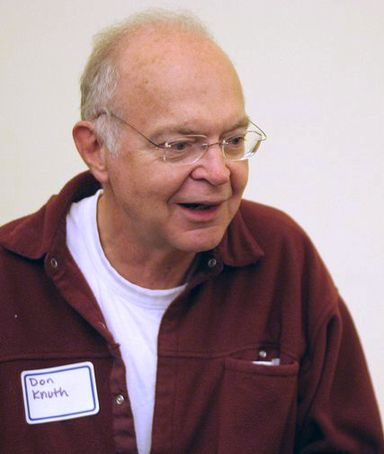
\includegraphics[scale=0.6]{images/Donald_Knuth.jpeg}
    \caption{克努斯博士,注:图片来源为克努斯博士的维基百科}
\end{figure}

由于克努斯博士此次在数学公式的排版上下足了功夫,就在他启动这项计划不久后,他收到了美国数
学协会 (American Mathematical Society, AMS) 的邀请,克努斯博士在此次邀请中汇报的内容
是“基于TeX排版,如何让计算机服务于数学”,这次汇报成功吸引了一大批数学家的目光。由于TeX
在数学公式排版方面的优秀表现,比如数学公式的自动间距调整,TeX后来摇身一变成为了书写数学
公式的“利器”。

为了提升TeX的开发质量,克努斯博士悬赏奖励任何能够在TeX中发现程序漏洞的人,也就是我们一般
认为的“找bug”。每一个bug的奖励金额从2.56美元(16进制的100美分)开始,以后每发现一个bug,
都会翻倍,直到327.68美元封顶。然而,克努斯博士从未因此而损失大笔金钱,因为TeX中的bug极
少,而真正发现bug的人在获得支票后往往因其纪念价值而不愿兑现。

随着时间的推移,TeX也派生出了很多优秀的软件,其中最著名的派生软件便是LaTeX。另外,美国
数学学会也发布了TeX版本的数学公式宏包,其中,以ams命名的宏包就有\emph{amsfonts}、
\emph{amsmath}、\emph{amssymb}等,这些宏包都可以在LaTeX上进行使用,在LaTeX上使用这
些宏包可以编辑出各种数学公式。

\begin{tcolorbox}[colback=red!5!white, colframe=red!50!black, title=参考资料]
    TeX的维基百科介绍: https://zh.wikipedia.org/wiki/TeX.
\end{tcolorbox}

\section{引领浪潮的\LaTeX }
\subsection{\LaTeX 的出现}
LaTeX是一款高质量的文档排版系统,LaTeX在读法上一般发作Lay-tek或者Lah-tek的音,而不
是大家普遍认为的Lay-teks。LaTeX的历史可以追溯到1984年,兰波特博士作为早期开发者在这一年
发布了LaTeX的最初版本。事实上,LaTeX完全是兰伯特博士的意外所得,他当年出于自己写书
的需要,在早先发布的文档排版系统TeX基础上新增了一些特定的宏包,为了便于自己日后可以重复
使用这些宏包,他将这些宏包进行规整,于是,便有了相应的标准宏包 (standard macro package)。
谁曾想,正是这些不经意间开发出来的宏包,在经过后续封装和发布使用手册之后,形成了LaTeX的
雏形。

\begin{figure}
    \centering
    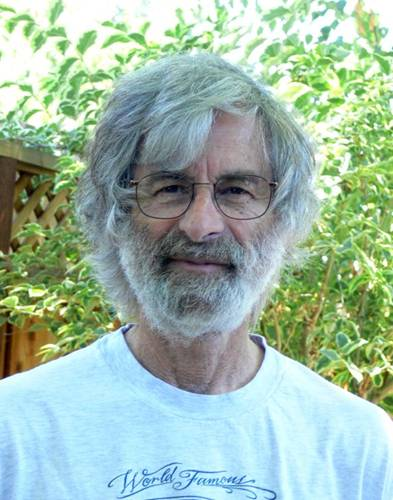
\includegraphics[scale=0.6]{images/Leslie_Lamport.jpeg}
    \caption{兰伯特博士,注:图片来源为兰伯特博士的维基百科}
\end{figure}

在很长一段时间里,LaTeX的版本其实没有多少大的更新,从技术层面来说,LaTeX实在没有什
么可供更新的地方了,它最初的面貌已趋近于完美且深入人心。LaTeX的最初版本是由兰伯特博士
于上世纪80年代初开发出来的,目前,广泛使用的版本LaTeX2e是在1994年发布的,发布后一直没有
大的更新,甚至发布后的首次更新出现在二十多年后的2020年。尽管LaTeX2e的后续版本更新工作早
在上世纪九十年代初就已经开展了,但时至今日,新版的LaTeX仍未进入人们的视野。从开发者兰伯
特博士的角度来看,开发LaTeX的目的是为了降低TeX的使用门槛、更容易地发挥TeX强大的排版功能,
提供一款高质量、解释性强的计算机程序语言,所以LaTeX最初的风格就是精简,这也是为什么LaTeX
在日后可供提升的地方不是很多的原因。

\subsection{\LaTeX 的特点}
由于种种原因,时至今日,TeX几乎淡出了人们的视线,不过我们现在依旧能看到:在使用LaTeX制作
文档时,通常需要创建一个以\emph{.tex}为拓展名的文件。对于很多人来说,日常制作各类文档的
首选可能是Word等软件,它简单好用、所写即所见,但当我们制作几十页甚至上百页的文档时,Word
的劣势就会展露无疑,因为我们需要投入大量的时间和精力来对文档内容进行排版。反观LaTeX,它
对文档的排版都是自动完成的,我们根本不需要像Word那样完全手动调整格式,另外,使用LaTeX插
入各种图形、表格、公式、文献时,相应的索引出错的可能性也非常小,这些优点都是Word所无法
比拟的。

在上个世纪80年代和90年代,LaTeX的用户群体非常庞大,然而,在世纪之交,随着微软推出的一系
列Windows操作系统快速发展,例如红极一时的XP系统,相应的办公软件Microsoft Office也以其
便捷性吸引了人们的视线,致使大量LaTeX用户转而使用Microsoft Office。即便如此,时至今日,
LaTeX的用户群体依旧十分庞大,这主要得益于LaTeX强大的文档排版能力,虽然LaTeX复杂的语法结
构、不容配置的编译环境让很多初学者望而却步,但LaTeX能让用户更专注于内容创作,而非锦上添
花的“排版”,这一显著特点契合了人们对质量和效率的追求,使得LaTeX在文档排版、论文撰写等方
面占有重要地位。在此基础上,具体来说,使得LaTeX历久弥新的关键可以归纳为以下五点:
\begin{enumerate}
    \item LaTeX是专门用于制作文档的计算机程序语言。在众多计算机程序语言中,LaTeX可以制
          作排版连贯性极好的专业文档。
    \item 独特的创作方式。尽管LaTeX沿用了TeX排版系统,但使用LaTeX制作文档时,内容创作
          和文档生成却是分开的,有需要的时候,我们可以预览创作的文档。因此,在创作的过程中,
          创作者不再像使用办公软件Word那样,既要关注创作内容,又要同步关注繁琐的排版和格式,
          使用LaTeX制作文档能在真正意义上让创作者专注于创作内容本身。更值得一提的是,当文档篇
          幅较大时,使用LaTeX无疑会让我们节省大量的时间和精力。
    \item 简单的逻辑结构。使用LaTeX制作文档时,创作者可以通过一些非常简单的逻辑结构进行
          创作,如chapter(章)、section(节)、table(表格)。因此,LaTeX的使用门槛并不像
          真正的程序语言那么高。很多人或许在使用LaTeX的过程中都不会用到for等基本的循环语句。
    \item 对数学公式以及特殊符号的支持程度。众所周知,LaTeX在开发之初,是作为数学和计算
          机相关研究人员的创作工具,这类群体喜欢使用LaTeX的原因无外乎是LaTeX可以通过一些简单
          的代码生成复杂的数学表达式和特殊符号。
    \item 编译以\emph{.tex}为拓展名的LaTeX文件后会得到一个PDF文档,PDF文档不存在跨
          平台、兼容性等问题,可以在各种操作系统上打开。
\end{enumerate}

当然,除了上述五点,实际上可能还有十分重要的一点,那就是LaTeX能够制作各类文档,从科技
论文、技术报告、著作、学位论文、幻灯片甚至到科技绘图一应俱全,当然它也支持嵌入图片、绘制
图形、设计表格、插入参考文献等。

从LaTeX的出现到当下,它已经形成了一套非常高效的文档制作环境:
\begin{itemize}
    \item 文档类型 (document class)。文档类型是文档排版样式的基调,这些类型包括
          文章 (article)、报告 (report)、幻灯片 (beamer)等,在.tex文件中申明文档类型后,
          我们就可以开始文档创作了。
    \item 宏包 (package)。它是LaTeX中的重要辅助工具,也可以把它理解为一般意义上的工具
          包。在使用时,调用宏包的基本命令为\emph{\textbackslash usepackage\{\}},举例来说,包含颜色命令的
          宏包为\emph{color},其调用语句为\emph{\textbackslash usepackage\{color\}}。随着LaTeX的发展,越来
          越多的宏包被开发出来,这些宏包能满足特定的需求(如制表、插图、绘图),同时也能让
          LaTeX代码变得更加简洁,我们只需要用简单的\emph{\textbackslash usepackage\{\}}命令就能调用
          所我们需要用到的宏包。
    \item 模板 (template)。LaTeX的发展催生了很多视觉和审美效果极好的模板,包括论文模板、
          幻灯片模板、报告模板甚至著作模板,这些模板在一定程度上能减少创作者在文档排版上的时间
          开销,也有很多学术刊物会给投稿作者提供相应的LaTeX模板。
\end{itemize}

通过对比LaTeX和Word,我们还会看到:
\begin{itemize}
    \item 第一,LaTeX的.tex源文件是无格式的,编译之后,根据特定的模板和指定的格式形成
          最终的PDF文档,因此,使用LaTeX制作各类文档能够很方便地切换模板和修改格式;
    \item 第二,LaTeX对公式、图表以及文献引用的支持是Word所无法比拟的,尤为特殊的是,
          当文献数量达到上百篇时,在Word中修改参考文献可能是“牵一发而动全身”,费时耗力,而
          LaTeX根据已经整理好的\emph{.bib}文件可自动完成文献引用和生成。
\end{itemize}

\subsection{\LaTeX 编辑器}
实际上,配置LaTeX环境包括两部分,即编译器和编辑器,对应的英文表达分别是editor和complier,
两者不是一回事。LaTeX编译器又称为LaTeX编译工具,可根据系统安装相应的编译工具:
\begin{itemize}
    \item Linux系统:可安装TeX Live,该编辑器拥有LaTeX编辑器;
    \item Mac OS系统:可安装Mac TeX,该编译器拥有完整的TeX/LaTeX环境和LaTeX编辑器;
    \item Windows系统:可安装MiKTeX或TeX Live,两者都拥有完整的TeX/LaTeX环境和LaTeX编辑器。
\end{itemize}

目前,我们可以接触到很多LaTeX编辑器,这些编辑器的界面大致有两部分组成,即LaTeX源码编译
区域和PDF文档预览区域。前面也提到了几款LaTeX编译器,但如果想要提高LaTeX的使用体验,以下
几款LaTeX编辑器比较受人推崇:
\begin{itemize}
    \item TeXworks:这是TeX Live自带的一款轻量级编辑器。
    \item TeXstudio:这款编辑器集代码编译与文档预览于一身。
    \item WinEdt:这是CTeX自带的一款编辑器。
    \item VS Code:这是微软推出的一款免费文本编辑器,功能包括文本编辑、日常开发等。
    \item Atom:这是一款开源的跨平台编辑器(GitHub网址为https://github.com/atom/atom),
          支持多种程序语言。
\end{itemize}

\section{应运而生的在线系统}
\subsection{\LaTeX 在线系统的出现}
上世纪80年代,LaTeX作为一件新生事物,在发布之初便引起了人们极大的兴趣,虽然在制作文档方
面拥有很多办公软件都无法比拟的强大优势,尤其在数学公式编写及高效排版上具有很大优势,但是
由于其较高的使用门槛(使用计算机程序语言进行编译)和安装成本(本地安装需要花费大量的时间
配置相应的环境),在很长一段时间里,LaTeX主要用户都是科研工作者。然而,LaTeX在线系统的
出现已实实在在地改变了这一尴尬局面。

随着信息技术快速发展、互联网深度普及,人们的工作生活方式也在发生着很大改变,很多过去安装
在本地的操作软件都被搬到了浏览器上,人们无须在个人计算机上安装各类办公软件就能进行办公,
这带来了极大的便利。不过这类在线系统也存在一些先决条件,例如,出于计算资源方面的考虑,通
常要求在线系统的类型不能是计算密集型,因为计算密集型的在线系统往往需要大量的计算资源作支
撑。反观LaTeX,尽管我们可以认为LaTeX是一种计算机程序语言,但实际上,其对计算资源的需求
并不是很大。

在过去,受网速限制,使用线上系统几乎是一件难以想象的事。然而,在线系统的兴起并非空穴来风,
一方面是目前的网速已经跟过去发生了质的变化,另一方面则是上网成本在急剧降低,互联网触手可
及,已经成为人们日常生活和工作中不可或缺的一部分。以前,我们可能已经习惯了在本地计算机上
安装和使用各类软件或者集成开发环境,不过以LaTeX为例,在本地计算机上安装的集成开发环境也
有很多缺陷:
\begin{itemize}
    \item 第一,我们需要为安装LaTeX编辑器腾出很大的存储空间;
    \item 第二,某些特定的宏包需要额外安装和配置,但安装过多宏包之后又会使LaTeX变得很臃肿,
          甚至是不友好;
    \item 第三,当我们在本地计算机使用LaTeX制作文档时,我们很难与合作者进行协同创作。
\end{itemize}

在这个背景下,一些成熟的LaTeX在线系统逐渐走进人们的视野,并受到很多用户的喜爱,其中,最
为著名的LaTeX在线系统便是\emph{overleaf.com}。这些LaTeX在线系统不仅支持各种语言、各种
拓展宏包等复杂的LaTeX环境,同时也支持实时编译和实时预览编译后的文档,就算是换一台电脑,
也丝毫不会影响创作过程,创作完成之后,可以选择下载压缩文件包(如.zip),也可以只导出PDF
文档,毫无疑问,这些人性化的设计都是为了让LaTeX更加便捷和高效。除此之外,现有的LaTeX在
线系统还提供大量的LaTeX模板库,科技论文、毕业设计、幻灯片、海报、简历等参考模板一应俱全,
就连LaTeX使用文档也数不胜数。

\begin{tcolorbox}[colback=red!5!white, colframe=red!50!black, title=在线系统 overleaf]
    Overleaf是一个初创的科技企业,它的主要业务是构建现代化协作创作工具,即LaTeX在线系统,
    旨在让科学研究变得更加便捷和高效。
    目前,Overleaf已合并另一款著名的LaTeX在线系统ShareLaTeX,在全球范围内拥有超过600万
    用户,这些用户大多是来自于高校和研究机构的研究人员、老师以及学生,只要打开网址overleaf.com,
    用户无需在本地计算机配置LaTeX环境就可以创建各种LaTeX项目。
    \tcblower
    关于Overleaf的介绍可参考https://www.overleaf.com/about。
\end{tcolorbox}

\begin{figure}
    \centering
    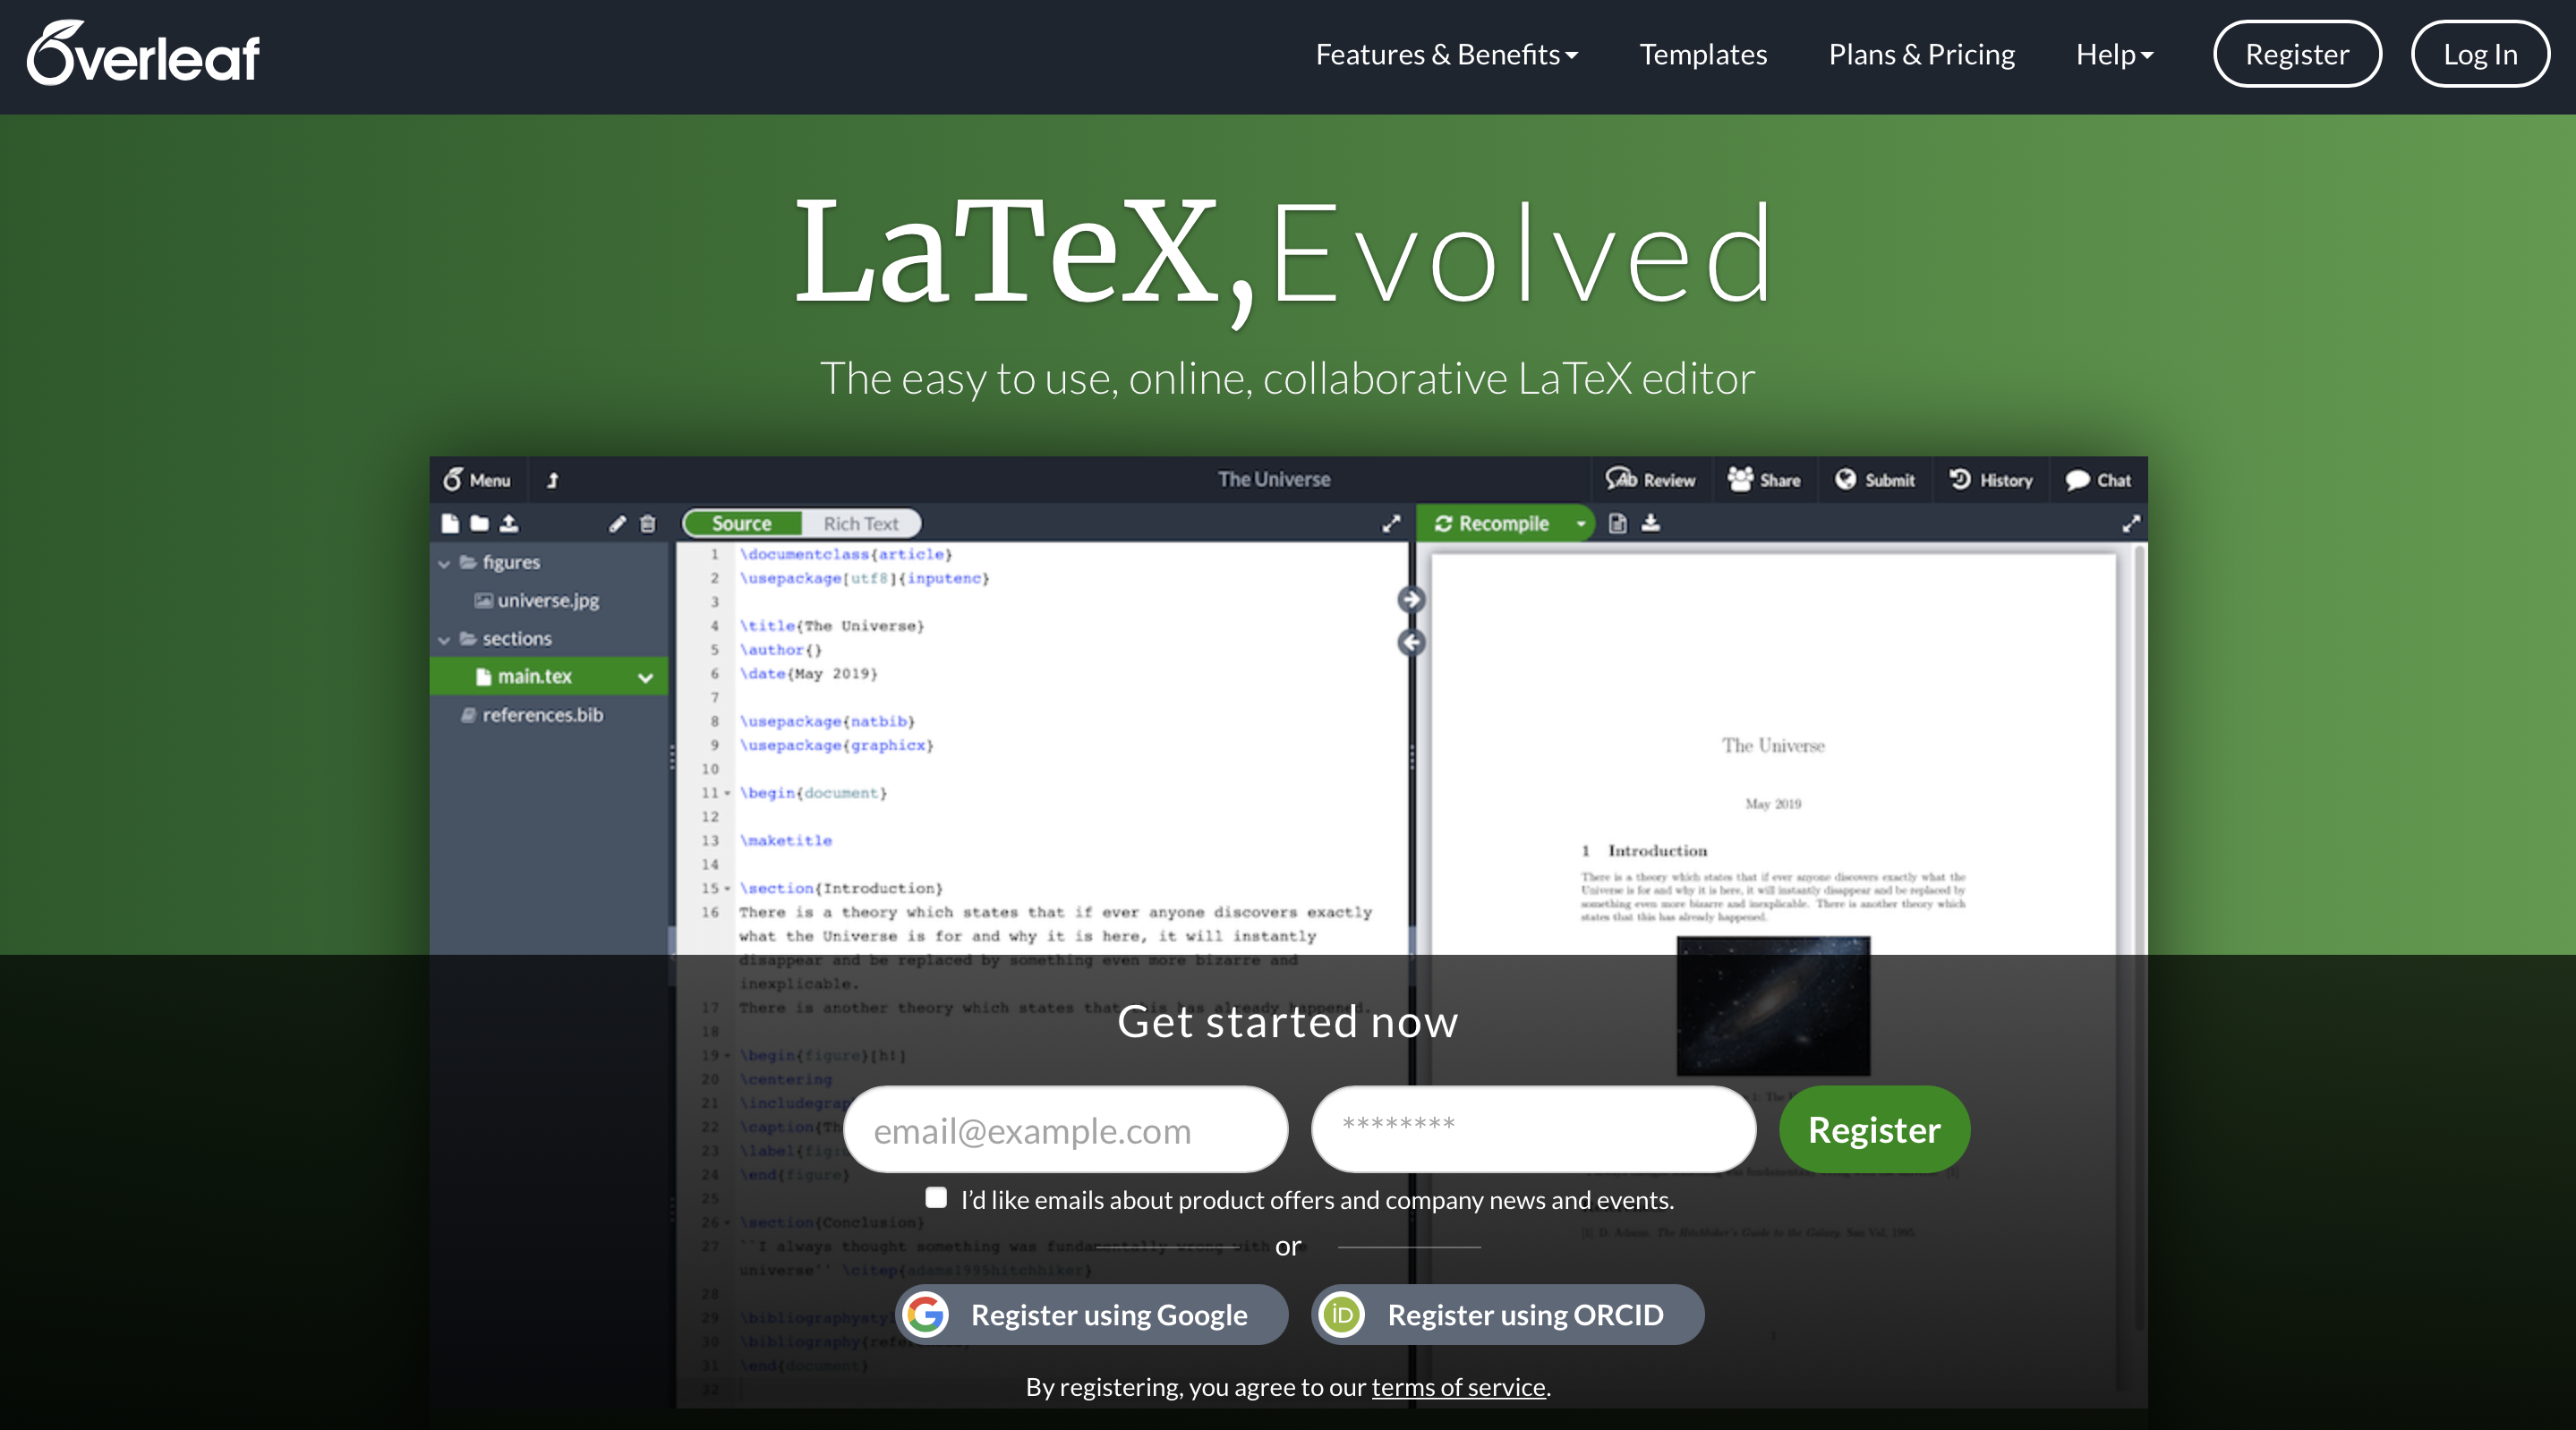
\includegraphics[width=\textwidth]{images/overleaf_webpage.png}
    \caption{Overleaf首页,图片来源于Overleaf官网}
\end{figure}

\subsection{\LaTeX 在线系统的特点}
以Overleaf为例,该LaTeX在线系统往往具备以下几点特征:
\begin{itemize}
    \item 免费和开源。可以免费注册和使用,不用下载和安装LaTeX编辑器,这一点对于初学者
          来说无疑是非常友好的;
    \item 使用简单。不管是在计算机、手机还是其他终端上,我们只需要使用浏览器打开overleaf.com
          就可以开始创作,另外,由于Overleaf界面非常简洁,所以用户使用起来也非常便利;
    \item 支持实时在线编辑。有各类LaTeX插件,编辑功能十分完善,且具有实时编译和预览功能;
    \item 支持在线协作。创作文档时,我们可以将文档项目分享给合作者进行协作,Overleaf支持实时编译,
          不会出现版本控制混乱等问题;
    \item 支持双向定位。可以在LaTeX代码与PDF文档内容之间进行双向定位;
    \item 提供丰富的模板库。Overleaf有着非常庞大的模板库,不仅有正式的学术论文、学位论文
          和书籍的参考模板,还有很多美观的报告、简历、幻灯片模板。就论文写作来说,用户可以在Overleaf
          官网找到众多期刊的LaTeX模板,根据使用说明,用户很容易就能用于撰写自己的论文;
    \item 提供大量的帮助文档。LaTeX提供了齐全的帮助文档,从LaTeX快速入门、基础操作到编译
          数学公式,应有尽有、一应俱全,且这些文档内容具有很强的实操性。
\end{itemize}

\begin{figure}
    \centering
    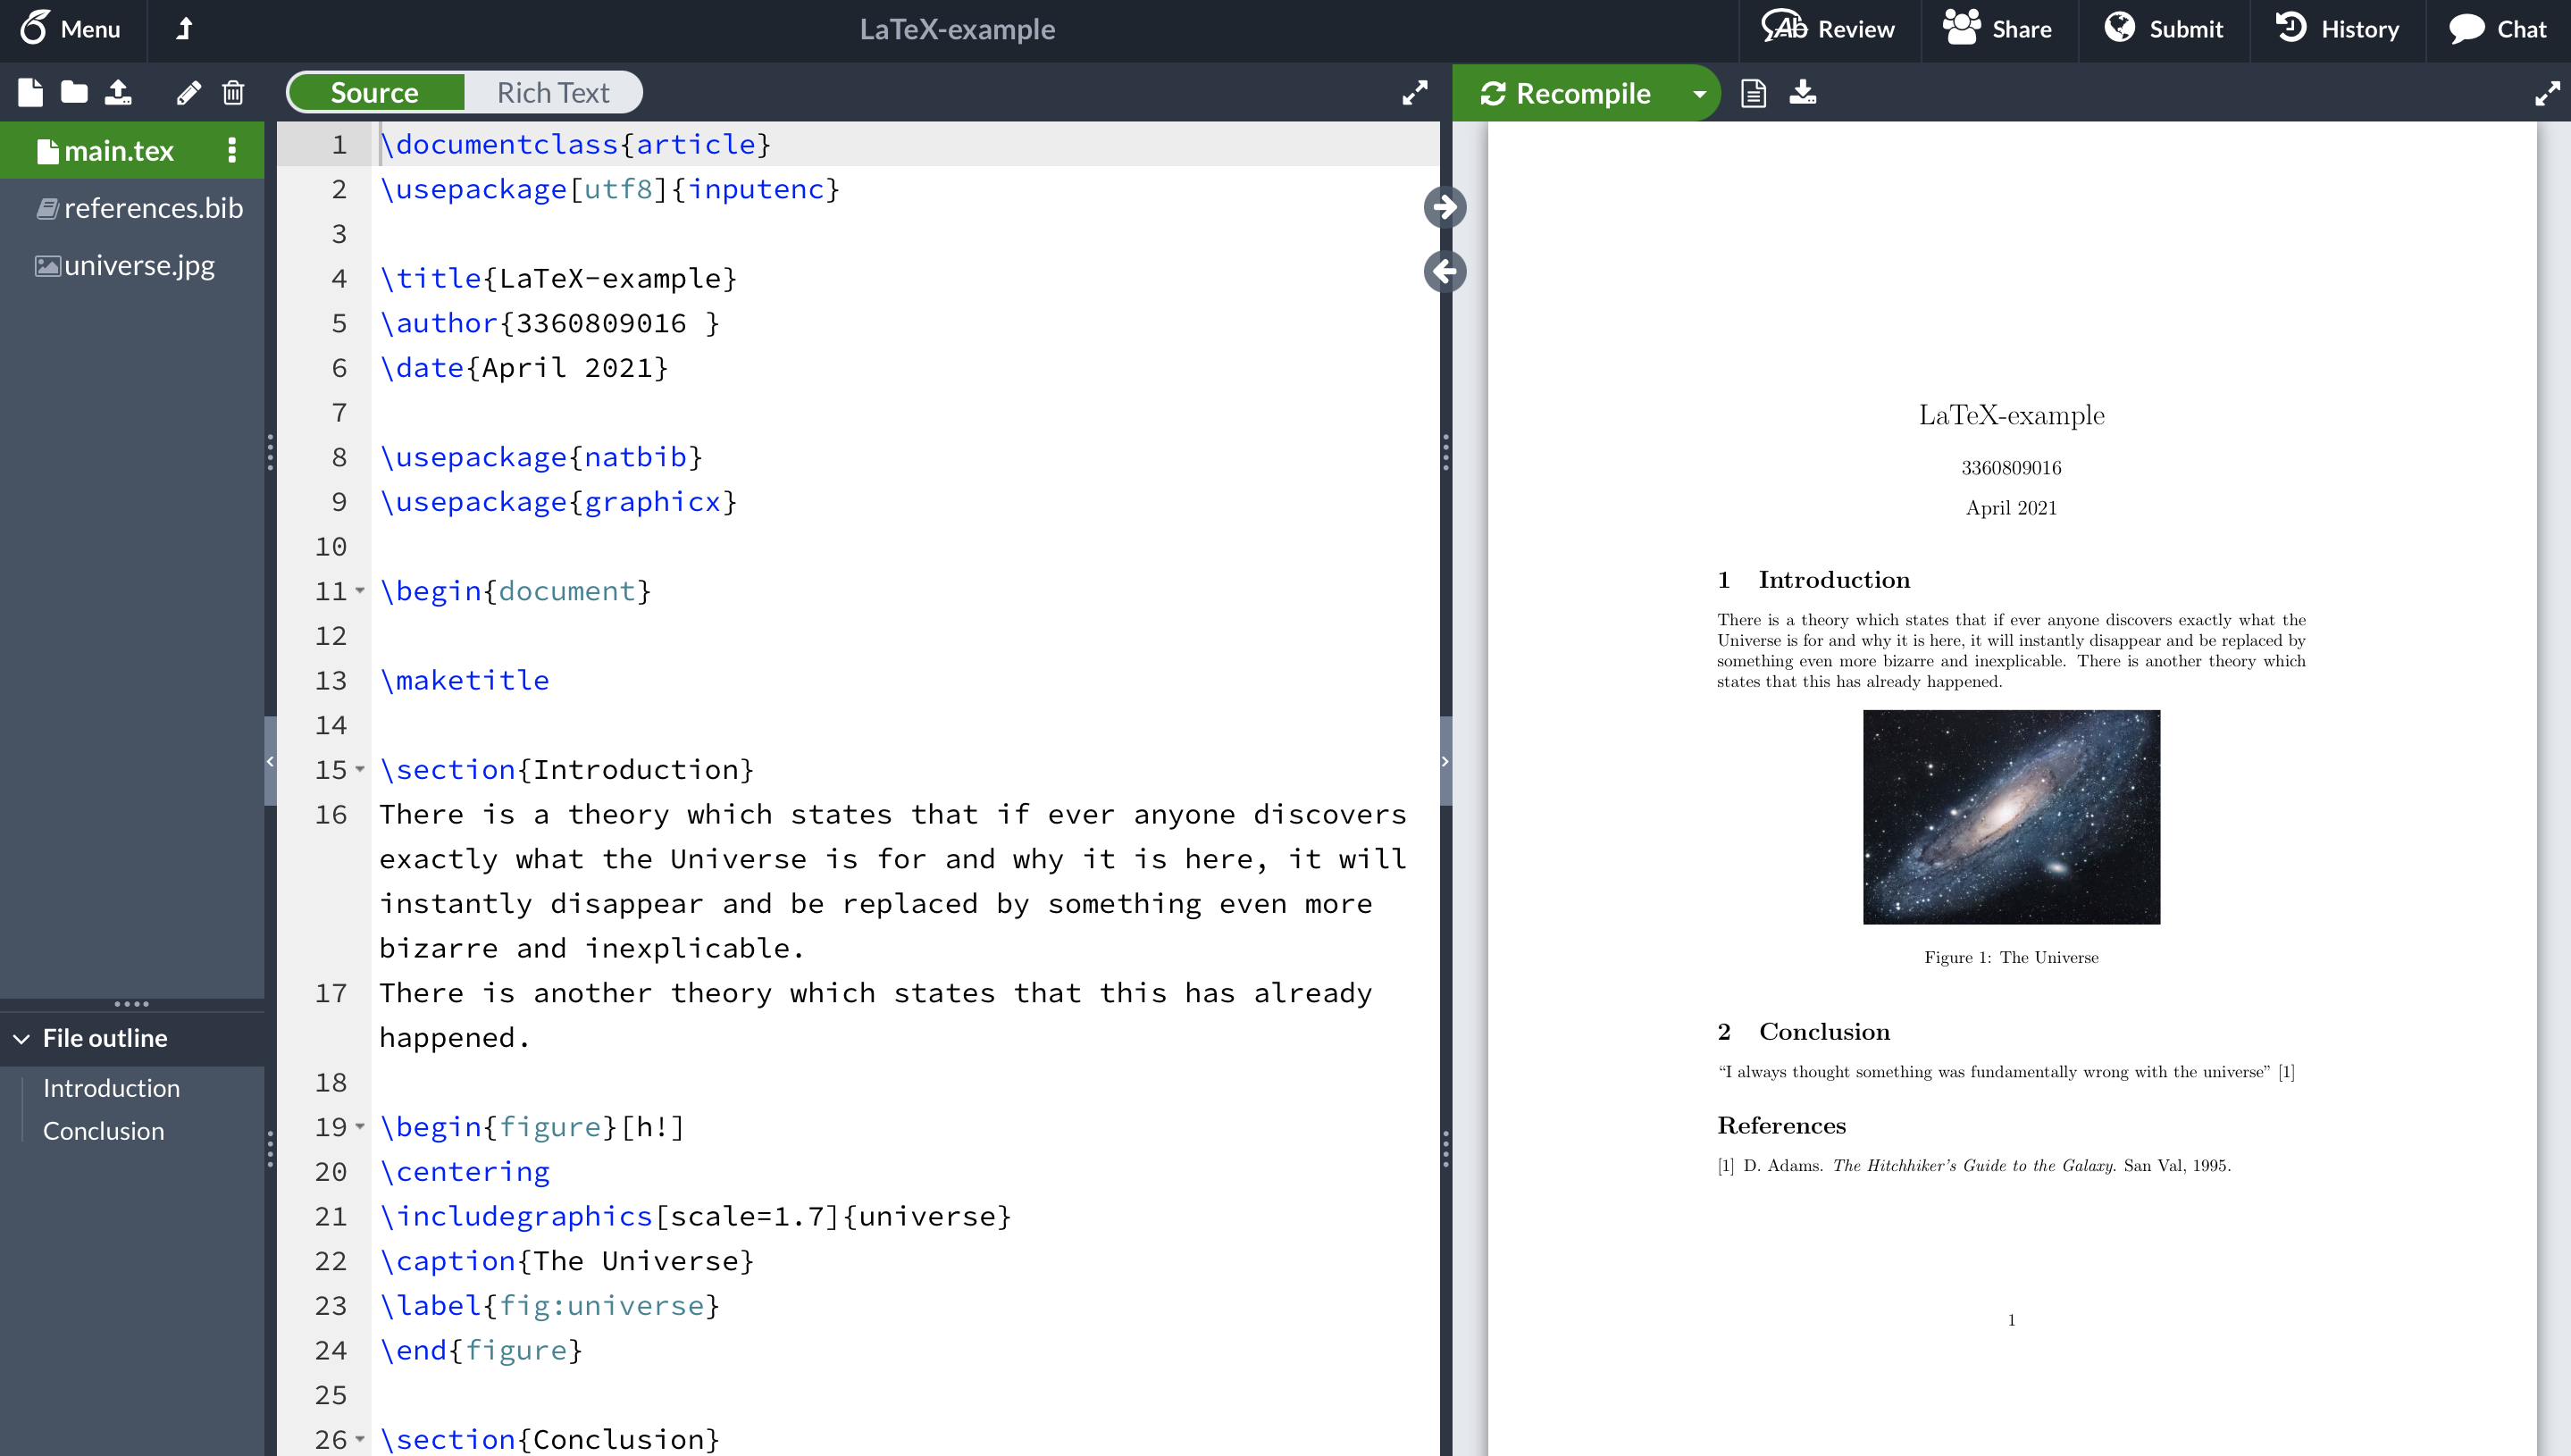
\includegraphics[width=\textwidth]{images/overleaf_example.png}
    \caption{Overleaf编辑器界面,主要由代码区域和文档预览区域组成}
\end{figure}

LaTeX在线系统的出现大大降低了LaTeX的使用门槛,也为用户省去了繁琐的安装和配置过程。其实,
LaTeX在线系统的出现并非个例,很多办公软件为迎合用户需求和时代发展趋势,陆续转变了产品研
发思路,包括微软在线Office系统、腾讯在线文档等在内的很多在线系统都走进了人们的视野,这些
在线系统能够在线备份、满足人们对随时随地办公的需求,在确保便捷和高效的同时,在线和共享的
理念正在潜移默化地影响着人们的办公模式。

\section{\LaTeX 问答社区}
在LaTeX刚被发布和推出的那个年代,相关资源如使用手册、教程等远没有今天这么丰富,同时,获
取渠道也没有今天这么便捷。在互联网触手可及的今天,我们能通过一个浏览器访问到各种相关学习
素材,遇到代码bug,也能在一些专业的问答社区找到最佳的解决方案。毫无疑问,对于今天的我们
来说,如何利用好互联网资源至关重要。

\subsection{问答社区的介绍}
对于从事计算机相关的技术人员来说,专业的技术问答社区往往是不可多得的资源,它能帮助很多技
术人员提升个人编程能力、学习新技术,同时解决一些技术困扰,例如解决编程时遇到的bug。对于
各类计算机程序语言而言,\emph{Stack Exchange}作为一个著名的技术问答社区,覆盖了大量编
程相关的技术问题和优质回答,就算是一些较为细致的问题,我们往往都能找到想要的答案。
Stack Exchange问答社区按计算机程序语言类型进行划分,我们所关心的LaTeX问答通常被分配在
TeX Stack Exchange社区(网址为https://tex.stackexchange.com/)。截至目前,
TeX Stack Exchange已经覆盖了关于TeX、LaTeX以及其他排版系统的用户在使用中遇到的诸多问题,
并且这些问题多与LaTeX相关。

\begin{tcolorbox}[colback=red!5!white, colframe=red!50!black, title=Stack Exchange]
    网址为https://stackexchange.com/,它与Stack Overflow问答社区在全球范围内拥有广泛的用户群体
\end{tcolorbox}

除了Stack Exchange这种涵盖了多种计算机程序语言的技术问答社区,LaTeX forum社
区(https://latex.org/forum/)是一个专门面向LaTeX的技术交流平台,它拥有非常活跃的用户
群体和丰富的问答资源,并拥有超过10万篇分门别类的技术帖子,我们可以根据浏览量从该平台一
览高频访问问题。

实际上,不管是LaTeX初学者还是高级用户,在遇到LaTeX使用问题时,去问答社区寻找解决方案都
是一种非常有效的方式。TeX Stack Exchange社区非常活跃,每天都会有大量关于LaTeX的问题和
回答,且每个问题下面的回答都会根据用户的认可度进行排序,回答一般比较细致。

\subsection{高频访问问题}
顾名思义,高频访问问题是指访问量较高的问题。LaTeX forum社区已经将众多问答帖子进行了分门
别类整理,针对某一特定话题,展开内容即可看到各类问题的访问情况。

\section{关于\LaTeX 的开源项目}
实际上,不管是TeX还是LaTeX,它们作为计算机程序语言是完全开源的,我们可以轻松获取到TeX
和LaTeX的源代码。近些年来,互联网催生了一些用户体验以及评价很好的开源社区,比如当下非常
受欢迎的开源平台GitHub,它们都在实实在在地影响着我们对于计算机技术开放的态度。开源社区
有很多优质的“仓库” (repository),这些仓库会提供诸如源代码、工具、案例甚至使用文档。与
LaTeX在线系统相似的是,这些开源社区非常支持协作功能,在有一些优质的仓库中,我们或许能看
到几十甚至上百个贡献者,“汇聚集体智慧”也是这些开源社区广受开发者青睐的一个重要原因。

\subsection{开源社区GitHub}
GitHub是一个面向开源项目及私有项目的云端托管平台,官方网址为http://github.com/,旨在为
开发者储存、管理代码以及控制代码的更新,只支持Git作为唯一的版本库格式进行托管。GitHub已
经走进人们的视野已经有十几年了,它于2008年4月10日正式上线,除了Git代码仓库托管和基本的
网页管理界面以外,还提供了在线文件编辑器、版本控制、协作报表等功能。截至2021年初,GitHub
在全球范围内拥有的注册用户已经超过5000万,托管项目的总量更是超过1亿,是很多开发者远程协作
的重要工具。2018年6月,GitHub被微软以75亿美元的价格收购。

GitHub本着开源、共享、协作的理念正影响着开发社区生态,吸引了包括微软和谷歌等国外技术巨头
在这里进行开源,另外,我们也能在GitHub上看到一些国内互联网企业的身影。实际上,GitHub开源
社区的项目类型及展现形式也异常丰富,既有大量的应用型项目,也有很多研究探索型项目。

为了方便开发者追踪整个开源社区的开发动态,GitHub根据计算机程序语言类型提供了趋势分析,这
个功能称为GitHub trending,它会定期更新趋势榜、帮助开发者追踪当下较为流行的GitHub仓库。

GitHub开源社区提供了很多关于LaTeX的优质开源项目,这些项目使得LaTeX的用户群体越来越广泛。
实际上, LaTeX在线系统Overleaf也是开源的,它托管在GitHub上,
网址为https://github.com/overleaf/overleaf。

为便于读者认识和掌握LaTeX,以下简单归纳一下关于LaTeX的各类开源项目。需要注意的是,优质的
开源项目是非常多的,限于篇幅,这里只列举一部分,感兴趣的读者不妨在GitHub平台上探寻更多
优质项目。

\subsection{学位论文\LaTeX 模板}
在GitHub开源社区中,我们可以找到很多国内外高校官方和非官方的学位论文LaTeX模板,学位论文
类型包括本科毕业设计、硕士学位论文和博士学位论文等。以下将列举一部分国内高校的学位论文
LaTeX模板开源项目:
\begin{itemize}
    \item 开源项目https://github.com/tuna/thuthesis提供了清华大学学位论文LaTeX模板,
          模板库涵盖本科综合论文训练、硕士论文、博士论文以及博士后出站报告,截至目前,已在
          GitHub上获得超过3000次标星。
    \item 开源项目https://github.com/mohuangrui/ucasthesis提供了中国科学院大学学
          位论文LaTeX模板,包括本科、硕士和博士学位论文模板,截至目前,已在GitHub上获得超
          过2000次标星。
    \item 开源项目https://github.com/mohuangrui/ucasthesis提供了中国科学院大学学
          位论文LaTeX模板,包括本科、硕士和博士学位论文模板,截至目前,已在GitHub上获得超
          过2000次标星。
    \item 开源项目https://github.com/ustctug/ustcthesis提供了中国科学技术大学学位
          论文LaTeX模板,包括本科毕业论文(设计)和研究生学位论文,截至目前,已在GitHub上
          获得近1000次标星。
    \item 开源项目https://github.com/TheNetAdmin/zjuthesis提供了浙江大学学位论文
          LaTeX模板,包含本科、硕士和博士学位论文模板,也提供了英文版的硕博士学位论文模板,
          截至目前,已在GitHub上获得近1000次标星。
    \item 开源项目https://github.com/dustincys/hithesis提供了哈尔滨工业大学学位论
          文LaTeX模板,包括本科、硕士、博士开题、中期和毕业论文,也提供了博后出站报告和英文
          毕业论文格式,截至目前,已在GitHub上获得近1000次标星。
    \item 开源项目https://github.com/x-magus/ThesisUESTC提供了电子科技大学毕业论
          文LaTeX模板,截至目前,已在GitHub上获得超过500次标星。
\end{itemize}

上述开源项目提供的学位论文模板绝大多数支持在LaTeX在线系统overleaf.com上直接进行编辑和使用。

\subsection{\LaTeX 绘制图形}
目前,LaTeX有很多关于绘制图形方面的宏包,这些宏包会提供图形的基本元素、颜色等。由于LaTeX
绘制出来的图形可以以PDF文档保存,所以一般不会出现分辨率不足等问题。这里对LaTeX绘制图形
相关的一些开源项目稍作整理:

\begin{itemize}
    \item 工具类:
          \begin{itemize}
              \item \emph{BayesNet}:用于绘制贝叶斯网络、图模型和因素图形的TikZ库。开源网址
                    为https://github.com/jluttine/tikz-bayesnet。一般而言,使用BayesNet绘制特定图
                    形时,需要使用以下两行命令调用该库:\emph{\textbackslash usepackage\{tikz\}}和
                    \emph{\textbackslash usetikzlibrary\{bayesnet\}}
              \item \emph{matlab2tikz}:将由Matlab代码绘制的图形转换成PGFPlots图形。开源网
                    址为https://github.com/matlab2tikz/matlab2tikz。
              \item \emph{tikzplotlib}:将由Python绘图工具matplotlib绘制的图形转换成PGFPlots
                    图形。开源网址为https://github.com/nschloe/tikzplotlib。
              \item \emph{svg2tikz}:将SVG图形转换成TikZ代码。开源网址为https://github.com/xyz2tex/svg2tikz。
          \end{itemize}
    \item 实例类:
          \begin{itemize}
              \item \emph{TeXample}:该项目提供了大量的TikZ绘图实例,开源网址为https://texample.net/tikz/。
              \item 开源项目https://github.com/walmes/Tikz提供了大约200个关于统计学的TikZ绘图实例。
              \item 开源项目https://github.com/MartinThoma/LaTeX-examples/tree/master/tikz提供了大约350个TikZ绘图实例。
              \item 开源项目https://github.com/PetarV-/TikZ提供了大量的Tikz绘图实例,囊括了各类神经网络模型的图形。
              \item TeX Stack Exchange社区中提供的可视化效果很好的TikZ科技绘图实例,网址
                    为https://tex.stackexchange.com/questions/158668/nice-scientific-pictures-show-off。
              \item 开源项目https://github.com/FriendlyUser/LatexDiagrams提供了大量的TikZ绘图实例,包括
                    流程图、图模型。
              \item 开源项目https://github.com/alemelis/tikz\_drawings提供了一些TikZ绘图实例。
          \end{itemize}
\end{itemize}

\subsection{\LaTeX 制作简历}
LaTeX可用于制作各类文档,这也包括简历。

\begin{itemize}
    \item 开源项目https://github.com/sb2nov/resume提供了简历模板。
    \item 开源项目https://github.com/xdanaux/moderncv提供了moderncv简历样式。
    \item 开源项目https://github.com/jankapunkt/latexcv提供了一些美观大方且容易使用的简历模板,支持包括中文在内的多种语言编译。
    \item 开源项目https://github.com/hijiangtao/resume提供了中文简历的模板。
\end{itemize}

\subsection{\LaTeX 制作幻灯片}
\begin{itemize}
    \item 开源项目https://github.com/matze/mtheme提供了现代风格主题的幻灯片模板。
    \item 开源项目https://github.com/wzpan/BeamerStyleSlides提供了很丰富的模板,包含了PowerPoint和Keynote两套格式。
    \item 开源项目https://github.com/XiangyunHuang/awesome-beamers提供了多种制作幻灯片的模版,同时也支持中文制作。
    \item 开源项目https://github.com/josephwright/beamer提供了多种风格的幻灯片模版。
\end{itemize}

\subsection{\LaTeX 制作海报}
\begin{itemize}
    \item 开源项目https://github.com/jkjaer/aauLatexTemplates提供了beamer海报模板。
    \item 开源项目https://github.com/mloesch/baposter提供了简洁的海报模版。
    \item 开源项目https://github.com/HolgerGerhardt/TeXTemplates提供了适合做学术报告的海报模版,同时也包含幻灯片模版。
\end{itemize}

\subsection{推荐指导本书的开源项目}
开源网址为https://github.com/xinychen/latex-cookbook。同时该作者还有图形绘制和幻灯片
制作的开源项目:
\begin{itemize}
    \item LaTeX图形绘制:https://github.com/xinychen/awesome-latex-drawing提供大
          量绘图实例,实例包括贝叶斯网络、框架图、流程图、机器学习模型示意图。
    \item LaTeX幻灯片制作:https://github.com/xinychen/awesome-beamer提供大量使用
          Beamer制作幻灯片的实例。
\end{itemize}

\begin{tcolorbox}[colback=red!5!white, colframe=red!50!black, title=参考资料]
    开源项目https://github.com/xiaohanyu/awesome-tikz。
\end{tcolorbox}

\section{\LaTeX 制作中文文档}
LaTeX最初只提供英文的编译环境,随着其在文档编辑领域的优势越来越深入人心,更多国家的学者
希望用到这一工具,因此出现了许多支持各国语言的工具包或编写环境,作为全世界使用人数最多的
语言,LaTeX有\emph{CJKutf8}宏包、\emph{CTEX}宏包等多种方式可以实现中文文档编辑,均能
在开源网站Overleaf中调用并实现中文文档制作。

\subsection{使用CJKutf8宏包}
\emph{CJKutf8}宏包提供了两种中文简体字体制作中文文档:使用\emph{\textbackslash begin\{CJK\}\{UTF8\}\{gbsn\}}
和\emph{\textbackslash end\{CJK\}}环境将以宋体(gbsn)制作文档,而使用\emph{\textbackslash begin\{CJK\}\{UTF8\}\{gkai\}}
和\emph{\textbackslash end\{CJK\}}环境则以楷体(gkai)制作文档内容。在默认的pdfLaTeX
编译环境中即可得到文档编译结果。

\emph{【例】}使用\emph{CJKutf8}红包制作中文文档:
\begin{lstlisting}[language=TeX, caption={CJKutf8示例}]
\documentclass{article}
\usepackage{CJKutf8}

\begin{document}

\begin{CJK}{UTF8}{gbsn} %字体是gbsn
你好,LaTeX!。
\end{CJK}

\end{document}
\end{lstlisting}

\subsection{使用CTEX宏包}
CJKutf8宏包只提供了两种字体,可选择的余地太小。如果想要使用更丰富的字体编辑 Latex 中文
文档,可以调用\emph{CTEX}宏包、并设置UTF8选项使其支持utf-8编码。在Overleaf中使用CTEX
宏包时,需要先将编译环境从\emph{pdfLaTeX}调整为\emph{XeLaTeX}。
\emph{【例】}使用\emph{CTEX}宏包制作中文文档:
\begin{lstlisting}[language=TeX, caption={CTEX示例}]
\documentclass[UTF8]{ctexart}

\begin{document}

{\kaishu 你好,LaTeX!(楷体)}

{\songti 你好,LaTeX!(宋体)}

{\heiti 你好,LaTeX!(黑体)}

{\fangsong 你好,LaTeX!(仿宋)}。

\end{document}
\end{lstlisting}

目前在Overleaf上已经出现了许多中文文档LaTeX模板,除了一些学位论文模板,一些中文学术期刊
如《计算机学报》也提供了科技论文的LaTeX模板。

\textbf{期刊模板:}
\begin{itemize}
    \item 《中国科学:信息科学》https://www.overleaf.com/project/5e99712a0916c900018d11af
    \item 《中国科学:信息科学》https://www.overleaf.com/project/5e99712a0916c900018d11af
\end{itemize}

\textbf{中文学位论文模板:}
\begin{itemize}
    \item 《浙江大学学位论文模板》https://www.overleaf.com/project/610fa05007d0073d5405a04f
    \item 《武汉大学博士学位论文模板》https://www.overleaf.com/project/610fa09e07d007fa5605a1e9
    \item 《武汉大学博士学位论文模板》https://www.overleaf.com/project/610fa09e07d007fa5605a1e9
    \item 《南京大学研究生毕业论文模板》https://www.overleaf.com/project/610fa1d007d00704c305a3eb
\end{itemize}

另外,开源项目https://github.com/MCG-NKU/NSFC-LaTex提供了国家自然科学基金申报书的LaTeX模板。

\chapter{\LaTeX 基础介绍}
\section{导言}
LaTeX作为专门用于制作文档的计算机程序语言,其语法规则是由命令 (command) 和环
境 (environment) 构成,基于一些基本命令,如\textbackslash usepackage\{\},我们能调用制
作文档所需的宏包。一般而言,在制作文档时,LaTeX的代码结构分为前导 (preamble) 和主
体 (body) 两部分,前导部分的代码主要用于申明文档类型、排版样式、所使用的宏包等;主体部
分主要用于确定标题、章节、目录等文章结构及创作文档内容。

掌握一些常用命令之后,我们便可上手编辑简单的文档。从功能上来说,LaTeX能满足人们对文档制
作多样性的要求。我们可以用LaTeX制作各类文档,包括科技文档、技术报告、学位论文、书籍著
作、幻灯片、个人简历、信件以及海报。不同的文档类型在文档大小、排版、章节样式方面略有不
同,所以在使用LaTeX制作文档时,我们首先需要对文档类型进行申明,然后再进行文档内容的创作。

本章节要介绍的内容主要包括:Latex语法规则、Latex代码结构、文档类型的介绍、简单文档的制
作以及全局格式的设置。

\section{\LaTeX 语法规则}
对于任何一种计算机程序语言,严格的语法规则都是让程序语言实现功能的保障。不同于一般性的计
算机程序语言,LaTeX的语法规则非常简单,是由命令和环境构成。在LaTeX中,不管是命令还是环
境,都离不开计算机符号反斜线\textbackslash,例如调用宏包会用到
\textbackslash usepackage\{宏包名称\},这里的花括号\{\}也是非常常用的一个符号。在调用宏包
后,命令的用法都是由宏包约定的。

\subsection{命令}
LaTeX中有很多命令,它们用法大同小异,功能却千差万别。既有申明文档类型的命令,如\textbackslash documentclass\{article\},
也有输入特殊符号的命令,例如\textbackslash copyright。一般而言,LaTeX中的命令通常由三
部分组成\textbackslash 命令名[可省略参数]\{不可省略参数\},具有以下特点:
\begin{itemize}
    \item 通常都是以反斜线作为开始,通过紧跟的既定字符(命令名)实现相应的功能,例
          如\textbackslash LaTeX和\textbackslash copyright可生成特殊字符。
    \item 一些命令需要申明一些参数,通过大括号中的不可省略参数进行申明,例如\textbackslash color\{blue\}
          命令中需要申明具体的颜色名称。
    \item 一些命令包括一些选项和一些参数一般情况下是默认的,有需要时可以通过中括号中的
          可省略参数进行调整,例如在\textbackslash documentclass[a4paper]\{article\}中,中
          括号[]作为额外的选项,既可以自行设置,也可以选择默认设置。
    \item 有些命令可以用反斜线作为终止,例如\textbackslash copyright。
\end{itemize}

\subsection{环境}
这里所说的“环境”是指编译环境,使用LaTeX时,当我们想要编译出期望的效果,例如列表、插入图
形、制作表格,我们就需要用到一些环境。举例来说,我们可以通过
\begin{lstlisting}[language=TeX]
    \begin{itemize}
        \item item 1 % 条目1
        \item item 2 % 条目2
    \end{itemize}
\end{lstlisting}

制作一个简单的无序列表,这里的\emph{itemize}表示无序列表环境,\emph{\textbackslash begin\{\}}
和\emph{\textbackslash end\{\}}表示环境的初始化和结束。当然,这些环境并非“一成不变”,我
们也可以设置一些参数,从而改变编译之后的文档效果,例如,可以通过
\begin{lstlisting}[language=TeX]
    \begin{spacing}{1.3}
        paragraph 1 % 第1段

        paragraph 2 % 第2段
    \end{spacing}
\end{lstlisting}
将两段话之间的行间距设置为1.3倍。

\emph{【例】}使用基本命令\textbackslash documentclass{article}和文档环境\textbackslash begin\{document\}
和\textbackslash end\{document\}创建一个简单文档。
\begin{lstlisting}[language=TeX]
    \documentclass{article}

    \begin{document}

    Hello, LaTeXers! This is our first LaTeX document.

    \end{document}
\end{lstlisting}

\subsection{宏包}
宏包是LaTeX的重要组成部分,用来扩展和增强LaTeX的功能,是支撑LaTeX实现一系列复杂文档编辑
和排版的关键所在。宏包与LaTeX的关系和浏览器插件与浏览器的关系类似,通过调用不同的宏包可
以实现一些复杂排版功能,例如插入表格、插入公式和特殊符号、插入程序源代码、设置文档样式等。
一个宏包通常会提供一组LaTeX命令,有些特殊命令只能在调用宏包后使用。在LaTeX中,调用宏包的
形式大同小异,如果想要使用某一特定宏包,最简单的办法就是用\textbackslash usepackage\{宏包名\}
命令对相应宏包进行调用。

\emph{【例】}使用\textbackslash usepackage\{color\}命令调用颜色宏包调整文本字体颜色。
\begin{lstlisting}[language=TeX]
    \documentclass{article}
    \usepackage{color} % 调用颜色宏包
    \begin{document}
    \textcolor[rgb]{1,0,0}{Hello, LaTeXers! This is our first LaTeX document.}
    \end{document}
\end{lstlisting}

\section{\LaTeX 代码结构}
在使用LaTeX进行文档编辑时,我们通常在拓展名为\emph{.tex}的源文件中书写代码,然后通过编译,生成
一个PDF格式的文档。LaTeX源文件的代码结构主要包含两个部分,即前导代码(preamble)和主体
代码(body),其结构示例如下:
\begin{lstlisting}[language=TeX]
    \documentclass[]{}

    ...... % 前导代码(preamble)

    \begin{document}

    ...... % 主体代码(body)

    \end{document}
\end{lstlisting}

\subsection{前导代码}
前导代码是指从源文件第一行代码到\textbackslash begin\{document\}之间的所有命令语句,
一般为LaTeX代码的第一部分。在前导代码部分,既可设置文档类型全局参数,包括字体大小、纸张
大小、文字分栏、单双面打印设置等,也可声明主体代码中需要用到的宏包,如插入图形、新增表格
所要用到的宏包。当全局格式没有特殊申明时,前导代码中的文档类型申明语句可以简写成\textbackslash documentclass\{B\},
其中,位置B的作用在于申明文档类型,如article(常规文档)、book(书籍)、report(报告)、
beamer(幻灯片)等。

下面以常规文档(article)为例,简要介绍各常用全局参数的设置方式。

\subsubsection{字体大小}
article类型文档字体大小默认为\emph{10pt},可在\textbackslash documentclass[可省参数]\{article\}
的中括号中根据需要设置成11pt和12pt。

通常,我们按照\textbackslash documentclass[fontsize = 12pt]\{article\}这样的形式设
置文档参数,有时候,为了方便起见,可以把文档类型申明做一定的简写,如\textbackslash documentclass[12pt]\{article\}。
需要注意的是,字体大小设置中的基本单位pt是英文单词point的缩写,是一个物理长度单位,
\textbf{指的是72分之一英寸,即1pt等于1/72英寸}。

\subsubsection{纸张大小}
article类型文档纸张大小默认为\emph{letterpaper},同样可在\textbackslash documentclass
    [可省参数]\{article\}的中括号中根据需要设置成\emph{a4paper}、\emph{a5paper}、\emph{b5paper}、
\emph{legalpaper}和\emph{executivepaper}。

\subsubsection{文字分栏}
article类型文档的文字分栏默认为\emph{onecolumn}(不分栏),也可以使用\emph{twocolumn}
参数设置为twocolumn(两栏)。

\subsubsection{单双面打印设置}
article类型文档打印时默认单面打印,同样可以使用\textbackslash documentclass[可省参数]
\{article\}中括号中的可选参数,通过添加\emph{twoside}参数进行双面打印的设置。

\begin{tcolorbox}[colback=red!5!white, colframe=red!50!black, title=文档属性设置小结]
    基于上面介绍可供调整的参数,我们可以进行任意无序组合,例如\textbackslash documentclass
        [a4paper, 11pt, twoside]\{article\}对应着文档类型为article、纸张大小为A4、字体大小为11pt的双面文档。
\end{tcolorbox}

\subsection{主体代码}
主体代码为\textbackslash begin\{document\}及\textbackslash end\{document\}之间所有
的命令语句和文本,一般由文档的创作内容构成,按照一般书写顺序,主要包含文档标题、目录、
章节、图表及具体文字内容等,通常配合一些基本命令的使用,来形成我们期望的文档。下面给出了
一个简单例子,让读者对如何制作一个包含标题、章节及其文字内容的简单文档能有一个比较粗略的
认识,更具体的语法命令我们将在后续章节中依次介绍。
\begin{lstlisting}[language=TeX]
    \documentclass{article}
    \title{LaTeX cook-book}

    \begin{document}
    \maketitle
    \section{Introduction}

    Hello, LaTeXers! This is our first LaTeX document.

    \end{document}
\end{lstlisting}

\section{文档类型介绍}
在LaTeX代码结构中,申明文档类型往往是制作文档的第一步,也是最基本的一步。事实上,不同
文档类型对应的文档样式略有不同,但制作不同类型的文档时,LaTeX中的绝大多数命令和环境却是
通用的,完成对文档内容的创作后,使用文档类型的申明语句可以让我们在不同类型的文档间切换自如。

\subsection{基本介绍}
对LaTeX熟悉的读者会知道,LaTeX实际上支持非常多的文档类型,例如,撰写科技论文会用到的
\emph{article}(常规文档)类型、制作演示文稿会用到的\emph{beamer}(幻灯片)类型。在众多文档类型中,
常见的文档类型包括\emph{article}(常规文档)、\emph{report}(报告)、\emph{book}(书籍)、\emph{beamer}(幻灯片)等,
如果使用支持中文编译的\emph{ctex}文档类型,还会有\emph{ctexart}(中文常规文档)、\emph{ctexrep}(中文报告)、
\emph{ctexbook}(中文书籍)等,文档类型会直接决定整个文档的样式和风格。

使用LaTeX制作文档时,申明文档类型是作为前导代码,其一般格式为:
\begin{lstlisting}
    \documentclass[A]{B}
\end{lstlisting}

在这一申明语句中,位置A的作用主要是设置控制全文的文档参数,我们可以调整全文的字体大小、
纸张大小、分栏设置等,因为各种文档类型都有一整套的默认参数,所以一般情况可以省略掉位置A。
在位置B,我们需要键入特定的文档类型,例如,\textbackslash documentclass[a4paper, 12pt]\{article\}
即表示申明一个纸张大小为A4、字体大小为12pt的常规文档。

以下将逐一介绍比较常用的三种文档类型,包括article(常规文档)、report(报告)、book(书籍)。
其中,report和book这两种文档类型的文档结构是一致的,可以使用的结构命令有\textbackslash part\{\}、
\textbackslash chapter\{\}、\textbackslash section\{\}、\textbackslash subsection\{\}、
\textbackslash subsubsection\{\}、\textbackslash paragraph\{\}、\textbackslash subparagraph\{\},
举例来说,包含颜色命令的而article文档类型中除了没有\textbackslash chapter\{\}这一结构命令
之外,其他都与report和book文档类型是一样的。

\begin{itemize}
    \item article是LaTeX制作文档时最为常用的一种文档类型,撰写科技论文往往会用到article文档类型。
    \item report主要是面向撰写各类技术报告的文档类型。
    \item book是用于制作书籍等出版物的文档类型。
\end{itemize}

\section{简单文档的制作}
LaTeX不但适合制作篇幅较大的文档,在制作篇幅较小的文档比如手稿、作业等时也十分方便。在LaTeX
的各类文档中,最为常用的文档类型为article (文章),以下将介绍如何制作一个简单文档。

\subsection{制作封面}
添加标题、日期、作者信息一般是在\textbackslash begin\{document\}之前,格式如下:
\begin{lstlisting}
    % 输入空格表示空的
    \title{标题}
    \author{作者名字}
    \date{日期} % 如果不设置则会自动设置为编译时的时间,如果不想展示日期则使用\data{}
\end{lstlisting}

如果要显示添加的相关信息,需要在\textbackslash begin\{document\}之后使用\textbackslash maketitle命令。

\subsection{开始创建文档}
在LaTeX中,以\textbackslash begin\{document\}命令为分界线,该命令之前的代码都统称为
前导代码,这些代码能设置全局参数。位于\textbackslash begin\{document\}和
\textbackslash end\{document\}之间的代码被视为主体代码,我们所创作文档的具
体内容也都是放在这两个命令之间。

\subsubsection{设置章节}
文档的章节是文档逻辑关系的重要体现,无论是中文论文还是英文论文都会有严谨的格式,章、节、段分明。
在LaTeX中,不同的文档类设置章节的命令有些许差别,\textbackslash chapter命令只在
book、report两个文档类中有定义,article类型中设置章节可以通过\textbackslash section\{name\}
及\textbackslash subsection\{name\}等简单的命令进行实现。

\subsubsection{段落}
段落是文章的基础,在LaTeX中,可以之间在文档中间键入空行文本作为段落,也可以使用
\textbackslash paragraph\{name\}和\textbackslash subparagraph\{name\}插入带标题的
段落和亚段落。

\subsubsection{生成目录}
在LaTeX中,我们可以通过一行简单的命令便可以生成文档的目录,即\textbackslash tableofcontents。
命令放在哪里,就会在哪里自动创建一个目录。默认情况下,该命令会根据用户定义的篇章节标题生
成文档目录。目录中包含\textbackslash subsubsection及其更高层次的结构标题,而段落和子段
信息则不会出现在文档目录中。注意如果有带\emph{*}号的章节命令,则该章节标题也不会出现在
目录中。如果想让文档正文内容与目录不在同一页,可在\textbackslash tableofcontents命令
后使用\textbackslash newpage命令或者\textbackslash clearpage命令。

类似对章节编号深度的设置,我们通过调用计数器命令\textbackslash mintinline\{tex\}\{\textbackslash setcounter\}
也可以指定目录层次深度。例如:
\begin{itemize}
    \item \textbackslash setcounter\{tocdepth\}\{0\} 目录层次仅包括part
    \item \textbackslash setcounter\{tocdepth\}\{1\} 目录层次深入到section
    \item \textbackslash setcounter\{tocdepth\}\{2\} 目录层次深入到subsection
    \item \textbackslash setcounter\{tocdepth\}\{3\} 目录层次深入到subsubsection,默认值
\end{itemize}

除此之外,我们还可以在章节前面添加\textbackslash addtocontents\{toc\}\{\textbackslash setcounter\{tocdepth\}\{\}\}
命令对每个章节设置不同深度的目录。另外还有一些其他的目录格式调整命令,如果我们想让创建的
目录在文档中独占一页,只需要在目录生成命令前后添加\textbackslash newpage;如果我们需要
让目录页面不带有全文格式,只需要在生成目录命令后面加上\textbackslash thispagestyle\{empty\}
命令;如果我们想设置目录页之后设置页码为1,则需要在生成目录命令后面加上\textbackslash setcounter\{page\}\{1\}
命令。

如果我们想要创建图目录或表目录,分别使用\textbackslash listoffigures、\textbackslash listoftables
命令即可,与创建章节目录的过程类似,这两个命令会根据文档中图表的标题产生图表目录,但不同
之处在于,图目录或表目录中所有标题均属于同一层次。

\emph{【例】}基于当前已掌握的知识的一个简单的article:
\lstinputlisting[language=TeX]{code/demo_1.tex}

\section{一些基本命令}
当我们运用LateX进行文档编辑时,需要用到一些基本命令。

\subsection{全局格式设置}
在前面,我们介绍了一些全局设置的命令在申明文档类型时可以进行的一些全局参数设置,使用方法
为在\textbackslash documentclass[可省参数]\{article\}的中括号中根据需要进行参数设置,
然而有些全局设置需要用到一些其他方法进行调整。例如,纸张方向、页边距等需要调用宏包进行参
数调整。同样地,我们以article类型文档进行举例说明。

\subsubsection{纸张方向}
article类型文档的纸张方向默认为\emph{portrait}(纵向),也可以设置成\emph{landscape}(横向)。
在文档中可以调用\emph{lscape}宏包中的\textbackslash begin\{landscape\} \textbackslash end\{landscape\}
环境将默认的纵向文档调整为横向。

\begin{tcolorbox}[colback=red!5!white, colframe=red!50!black,
        title=How to change certain pages into landscape/portrait mode]
    https://tex.stackexchange.com/q/337/227605
\end{tcolorbox}

\subsubsection{页边距}
article类型文档的页边距可以通过调用\emph{geometry}宏包进行调整
\begin{lstlisting}[language=TeX]
    \usepackage{geometry} % 使用页面设置宏包
    \geometry{left=3.0cm,right=3.0cm,top=2.5cm,bottom=2.5cm} % 设置页边距
\end{lstlisting}

\subsubsection{章节标题的字体格式}
article类型文档的章节标题的字体格式可以通过调用\emph{sectsty}宏包进行调整。

一些设置例举:
\begin{lstlisting}
    \usepackage{sectsty}
    \sectionfont{\fontfamily{phv}\fontseries{b}\fontsize{11pt}{20pt}\selectfont} % 一级标题字体格式设置
    \subsectionfont{\fontfamily{phv}\fontseries{b}\fontsize{11pt}{20pt}\selectfont} % 二级标题字体格式设置
    \subsubsectionfont{\fontfamily{phv}\fontseries{b}\fontsize{11pt}{20pt}\selectfont} % 三级标题字体格式设置
\end{lstlisting}

\subsubsection{图、表、公式格式全局设置}
当我们需要批量设置图、表及公式的格式时,可以通过调用caption宏包进行全局设置。
例:
\begin{lstlisting}[language=TeX]
    \usepackage[labelfont=bf,labelsep=period,font={bf,sf,normalsize}]{caption}
\end{lstlisting}

\begin{tcolorbox}[colback=red!5!white, colframe=red!50!black,
        title=Changing/Defining Fonts for an Entire Document]
    https://tex.stackexchange.com/q/337/227605
\end{tcolorbox}

\subsubsection{自定义命令全局设置}
有时,我们需要也可以使用一些自定义命令来更改全局设置。例如在更改整个文档的字体格式时,
我们也可以使用:
\begin{lstlisting}[language=TeX]
    \renewcommand{\sfdefault}{\fontencoding{T1}\fontfamily{phv}\selectfont}
    \renewcommand{\familydefault}{\sfdefault}
\end{lstlisting}
等命令。

在更改目录标题时,我们可以使用:
\begin{lstlisting}[language=TeX]
    \renewcommand{\contentsname}{new name of Contents}
\end{lstlisting}

\chapter{文本编辑}
文本编辑是组成科技论文或科技报告的重要主要内容。而对于论文或报告中,简洁美观的文本对于阅
读者的理解以及感受是非常重要的。因此,我们需要认真学习在Latex中如何编辑出清晰明了的文本
内容。

文本编辑的内容一般包括文本章节的设定、文本段落的编辑、文字格式的编辑、列表的创建、页眉页
脚和脚注的创建。其中文本段落的编辑又包括段落首行缩进、段行间距、段落对齐方式的调整等,而
文字的编辑主要包括字体样式的调整、字体大小的调整、字体颜色的调整、字体本身的设定、字体中
的下划线和删除线、以及一些特殊字符的书写等内容。

列表的创建是方便读者对文本进行阅读,而这一类文本中的内容一般处于并列关系。合适的列表可以
方便读者知道文本的框架和内容关系。列表内容主要包括无序列表、排序列表、阐述性列表和自定义
列表格式。对于文本编辑,页眉页脚和脚注是很重要的,页眉一般可以用于显示题目或者章节名称等
提醒内容,而页脚可以显示文本页码等重要信息,脚注可以用于备注一些重要特别内容,如作者个人
信息以及项目资助信息等。本章将详细介绍文本编辑的相关内容,学好文本编辑有助于我们完成一个
阅读性更好的高质量文档。

\section{创建标题部分、摘要及关键词}
文档主体代码是指位于document环境的部分。在文档正文章节内容及目录之前,一般先创建标题部
分(包括文档标题、作者和日期)、摘要、以及关键词信息,这也是文档主体代码中最开始的部分。
下面分别介绍这部分的创建过程。

\subsection{创建标题部分}
\begin{itemize}
      \item 使用\verb|\|title\{\}命令设置文档标题,对于较长的文档标题,
            可以使用\verb|\\|对标题内容进行分行。
      \item 使用\verb|\|author\{\}命令设置作者,如果有多个作者,作者之间可以使
            用\verb|\|and进行分隔。
      \item 使用\verb|\|date\{\}命令设置日期信息,在实际使用时,有时需要省略日期
            信息,那么在\{\}中不写任何内容即可。如果想要使用默认值(当前日期),则应使用\verb|\|date命令。
      \item 使用\verb|\|maketitle命令完成标题部分的创建。
\end{itemize}

仅仅执行上述三行语句无法在文档编译时生成标题部分,还必须在之后加上\verb|\|maketitle
命令,表示对标题部分内容进行排版才能真正实现标题部分的创建。

\subsection{创建摘要及关键词}
在LaTeX中,使用\emph{abstract}环境撰写文档摘要部分,并在其后使用\verb|\|textbf\{\}
命令设置文档关键词。

\section{创建章节}
在制作文档时,不管是学术论文还是书籍,都需要创建章节来优化文章的层次结构。LaTeX提供了不
同层次章节的创建命令,从高到低包括:使用\verb|\|part\{\}命令创建不同篇、使用\verb|\|chapter\{\}
命令创建不同章、使用\verb|\|section\{\}命令创建一级节、使用\verb|\|subsection\{\}命令
创建二级节、以及使用\verb|\|subsubsection\{\}命令创建三级节。各篇章节的标题填写在\{\}中。

对于article类型文档,可以调用上述除了\verb|\|chapter\{\}命令之外的其他章节命令。而在
book、report类型文档中,则可以调用上述所有章节命令。

在撰写学术论文时,不同出版商所要求的章节标题格式可能是不一样的。因此,我们需要根据不同需
要调整章节标题的格式。

\begin{itemize}
      \item 自动编号与取消自动编号:在LaTeX中使用上述命令创建章节时,默认会对各章节进行自
            动编号。如果用户想要对某章节取消自动编号,只需要在章节命令后加上星号即可,如\verb|\|section*\{\}
            命令。
      \item 设置章节自动编号深度:用户也可以通过在导言区使用\verb|\|setcounter\{secnumdepth\}\{\}
            计数器命令设置章节自动编号深度,从而达到批量取消自动编号的效果。在\{\}中填写编号深度
            值,编号深度值从0开始设置,表示章节自动编号深入层次:
            \begin{itemize}
                  \item \verb|\|setcounter\{secnumdepth\}\{0\}表示自动编号章节层次仅包括\verb|\|part和\verb|\|chapter;
                  \item \verb|\|setcounter\{secnumdepth\}\{1\}表示自动编号层次深入到\verb|\|section级;
                  \item \verb|\|setcounter\{secnumdepth\}\{2\}表示自动编号层次深入到\verb|\|subsection级;
                  \item \verb|\|setcounter\{secnumdepth\}\{3\}表示自动编号层次深入到\verb|\|subsubsection级,默认值。
            \end{itemize}
      \item 改变字体样式:对于改变字体样式,我们需要使用\emph{titlesec}宏包,使用该宏包中
            的命令\verb|\|titleformat*\{\}\{\}来改变字体样式。
\end{itemize}

当然,有时我们也会遇到一些出版商要求我们将标题居中显示,在LaTeX的article文档类型中,我们
可以调用\emph{sectsty}宏包,并用到\verb|\|sectionfont\{\verb|\|centering\}使标题居中。

\section{生成目录}
章节目录一般在摘要之后创建,使用\verb|\|tableofcontents命令即可。命令放在哪里,就会在
哪里自动创建一个章节目录。默认情况下,该命令会根据用户定义的篇章节标题生成文章目录,目录
中将包含\verb|\|subsubsection及其更高层次的结构标题。但对于带星号的章节命令,其章节标
题不会出现在目录中。

根据需要,用户可以对目录格式进行各项调整。

\subsection{调整章节层次深度}
在前一节中我们介绍了使用\verb|\|setcounter\{secnumdepth\}\{\}计数器命令调整章节自动编
号深度,类似地,我们可以通过在导言区使用\verb|\|setcounter\{tocdepth\}\{\}命令指定目录
中的章节层次深度。
\begin{itemize}
      \item \verb|\|setcounter\{tocdepth\}\{0\},目录层次仅包括part和chapter;
      \item \verb|\|setcounter\{tocdepth\}\{1\},设置目录层次深入到section级;
      \item \verb|\|setcounter\{tocdepth\}\{2\},设置目录层次深入到subsection级;
      \item \verb|\|setcounter\{tocdepth\}\{3\},设置目录层次深入到subsubsection级,默认值;
\end{itemize}

上面的语句可以为所有章节指定了相同的目录层次深度。此外,我们也可以为每个章节设置不同的目录
层次,具体是通过在每个章节创建命令前,使用\verb|\|addtocontents\{toc\}{\verb|\|setcounter\{tocdepth\}\{\}\}
命令为该章节指定目录层次深度。

\subsection{给目录设置别名}
对于章节标题特别长的情况,直接在目录中显示完整标题显然可视化效果不佳,因此需要为长章节标题
设置一个比较短的“目录别名”。通过这种设置,在正文中可以显示完整标题,而在目录中将显示“短标题”。
为此,只需要在章节创建命令中添加目录别名选项即可。例:\verb|\|section[FS]\{First Section\}

\subsection{给目录设置链接}
如果想要为目录中的章节引用添加链接,使得点击链接后就能跳转到相应章节所在页面,那么只需要
在导言区调用\emph{hyperref}宏包。如果设置colorlinks=true选项,此时文档中章节引用及其
它交叉引用均会被自动添加链接(添加了链接的引用将显示为红色)。

\section{编辑段落}
\subsection{段落首行缩进}
许多出版社要求文章段落必须首行缩进,若想调整段落首行缩进的距离,可以使用\verb|\|setlength\{\verb|\|parindent\}\{长度\}
命令,在\{长度\}处填写需要设置的距离即可。例:\verb|\|setlength\{\verb|\|parindent\}\{2em\}

当然,如果不想让段落自动首行缩进, 在段落前使用命令\verb|\|noindent即可。

需要注意的是,在段落设置在章节后面时,每一节后的第一段默认是不缩进的,为了使第一段向其他
段一样缩进,可以在段落前使用\verb|\|hspace*\{\verb|\|parindent\}命令,也可以在源文件的
前导代码中直接调用宏包\verb|\|usepackage\{indentfirst\}。

\subsection{段落间距调整}
在使用LaTeX排版时,有时为了使段落与段落之间的区别更加明显,我们可以在段落之间设置一定的
间距,最简单的方式是使用\verb|\|smallskip、\verb|\|medskip和\verb|\|bigskip等命令。

\begin{tcolorbox}[colback=red!5!white, colframe=red!50!black,
            title=设置段落间距的几种方法]
      https://latex.org/forum/viewtopic.php?f=44\&t=6934
      \tcblower
      https://tex.stackexchange.com/questions/41476/lengths-and-when-to-use-them
\end{tcolorbox}

\subsection{段落添加文本框}
有时因为文档没有图全都是文字,版面显得极其单调。如果想让版面有所变化,可以通过给文字加边
框来实现对段落文本新增边框。在LaTeX中,我们可以使用\verb|\|fbox\{\}命令对文本新增边框。

\begin{tcolorbox}[colback=red!5!white, colframe=red!50!black,
            title=How to put a box around multiple lines?]
      https://latex.org/forum/viewtopic.php?f=44\&t=4117
\end{tcolorbox}

\subsection{段落对齐方式调整}
LaTeX默认的对齐方式是两端对齐,有时在进行文档排版的过程中,我们为了突出某一段落的内容,
会选择将其居中显示,在LaTeX中,我们可以使用\emph{center}环境对文本进行居中对齐。另外还有一些出
版商要求文档是左对齐或者右对齐,这时我们同样可以使用\emph{flushleft}环境和\emph{flushright}
环境将文档设置为左对齐或右对齐。

\section{文字编辑}
文字编辑是制作文档非常重要的一部分,主要关注如何调整字体样式、字体设置、增加下划线、突出
文字、调整字体大小、调整对齐格式等内容。

\subsection{调整字体样式}
调整文字的样式有很多对应的命令,这些命令包括\verb|\|textit、\verb|\|textbf、\verb|\|textsc、\verb|\|texttt,
在使用的过程中,需要用到花括号\{\}。具体而言,\verb|\|textit对应着斜体字,\verb|\|textbf对应着粗体字,
\verb|\|textsc对应着小型大写字母,\verb|\|texttt对应着打印机字体(即等宽字体)。

除了这几种字体样式,有时候,如果想对文本中的英文字母进行全部大写,可用\verb|\|uppercase和
\verb|\|MakeUppercase两个命令中的任意一个。

一般而言,当我们需要对段落、句子、关键词等做特殊标记时,往往会用到上述几种字体样式,其中,
打字机字体主要用于代码的排版,有时候,如果需要添加一个网站,通常也会选用打字机字体对文本进行
突出,例如\verb|\|texttt\{https://www.overleaf.com\}。

\subsection{调整字体大小}
字体大小的设置一方面可以在申明文档类型的命令\verb|\|documentclass[]\{\}中指定具体的字体
大小(如11pt、12pt)来实现,另一方面也可以通过一些简单的命令来调整。
\begin{lstlisting}[language=TeX]
      \documentclass[12pt]{article}
      \begin{document}

      Produce {\tiny tiny word}

      Produce {\scriptsize script size word}

      Produce {\footnotesize footnote size word}

      Produce {\normalsize normal size word}

      Produce {\large large word}

      Produce {\Large Large word}

      Produce {\LARGE LARGE word}

      Produce {\huge huge word}

      Produce {\Huge Huge word}

      \end{document}
\end{lstlisting}

在这里,这些命令对应的字体依次是从小到大。当然,这些命令也有另外一种使用方法,以
\verb|\|large、\verb|\|Large、\verb|\|LARGE为例,我们可以使用\verb|\|begin\{\} \verb|\|end\{\}
语句来实现对字体的加大:
\begin{lstlisting}[language=TeX]
      \documentclass[12pt]{article}
      \begin{document}

      Produce \begin{large}large word\end{large}

      Produce \begin{Large}large word\end{Large}

      Produce \begin{LARGE}large word\end{LARGE}

      \end{document}
\end{lstlisting}

\subsection{调整字体颜色}
一般而言,文本默认的颜色是黑色,但有时候,我们可以根据需要改变字体的颜色,这通过LaTeX一些
拓展的宏包就可以实现,例如\emph{xcolor}。

使用颜色宏包时,我们也可以根据需要自定义颜色,相应的命令为\verb|\|definecolor\{A\}\{B\}\{C\},其中
位置A是颜色标签,位置B是制定颜色系统为RGB(英文缩写RGB是红色、绿色和蓝色三种颜色的英文
单词首字母),位置C是具体的RGB数值。
\begin{lstlisting}[language=TeX]
      \documentclass[12pt]{article}

      \usepackage{color}
      \definecolor{kugreen}{RGB}{50, 93, 61}
      \definecolor{kugreenlys}{RGB}{132, 158, 139}
      \definecolor{kugreenlyslys}{RGB}{173, 190, 177}
      \definecolor{kugreenlyslyslys}{RGB}{214, 223, 216}

      \begin{document}

      This is a simple example for using \LaTeX.

      {\color{kugreen}This is a simple example for using \LaTeX.}

      {\color{kugreenlys}This is a simple example for using \LaTeX.}

      {\color{kugreenlyslys}This is a simple example for using \LaTeX.}

      {\color{kugreenlyslyslys}This is a simple example for using \LaTeX.}

      \end{document}
\end{lstlisting}

\subsection{字体设置}
不管是英文还是中文,我们都会越到各种各样的字体,因此,使用LaTeX编译出想要的字体对于整个
文档也非常重要。对于英文文档的编译,一般会用宏包fontspec设置具体的字体,调用格式为\verb|\|usepackage\{fontspec\},
需要说明的是,这个宏包只能设置英文的字体。例如:
\begin{lstlisting}[language=TeX]
      \setmainfont{Times New Roman}
      \setsansfont{DejaVu Sans}
      \setmonofont{Latin Modern Mono}
      \setsansfont{[foo.ttf]}   
\end{lstlisting}

如果文档输入的是中文,首先需要申明文档类型为ctex中的ctexart、ctexrep之类的。

在LaTeX中,编译文档一般默认的英文字体为Computer Modern,如果要将其调整为其他特定类型的
字体,可以在前导代码中使用各种字体对应的工具包。

\begin{tcolorbox}[colback=red!5!white, colframe=red!50!black,
            title=更多字体设置参考]
      https://www.overleaf.com/learn/latex/Font\_typefaces
\end{tcolorbox}

\subsection{下划线与删除线}
有时候,为了突出特定的文本,我们也会使用到各种下划线。最常用的下划线命令是\verb|\|underline,
然而,这个命令存在一个缺陷,即当文本过长,超过页面宽度时,下划线不会自动跳到下一行,因此,
我们需要用到一个叫\emph{ulem}的宏包,使用这个宏包中的命令\verb|\|uline可以增加单下划线,
使用\verb|\|uuline可以增加双下划线,而使用\verb|\|uwave则可以增加波浪线。

\begin{lstlisting}[language=TeX]
      \documentclass[12pt]{article}
      \usepackage{ulem}
      \begin{document}

      Generate \underline{underlined} text. \\     % 生成带下划线的文本(使用\underline命令)

      Generate \uline{underlined} text. \\         % 生成单下划线的文本(使用\uline命令)

      Generate \uuline{double underlined} text. \\ % 生成单下划线的文本

      Generate \uwave{wavy underlined} text. \\    % 生成波浪线的文本

      \end{document}
\end{lstlisting}

删除线是文字中间划出的线段,常见于文档的审阅。在LaTeX中,我们可以使用宏包\emph{soul}中的\verb|\|st
命令生成删除线。

下划线在LaTeX环境中属于特殊字符,如果需要在文本中使用下划线,则需要家上反斜线进行转义,例:
\begin{lstlisting}[language=TeX]
      \documentclass[12pt]{article}
      \begin{document}

      This\_is\_text\_with\_underscores.

      \end{document}
\end{lstlisting}

\subsection{特殊字符}
在LaTeX中,有很多特殊字符的编译需要遵循一定的规则,例如:
\begin{itemize}
      \item 反斜杠 (backslash) 符号是LaTeX中定义和使用各类命令的基本符号,如果要在文档
            中编译出反斜杠,可使用\verb|\|textbackslash;
      \item 百分号通常用于注释代码,如果要在文档中编译出百分号,可使用\verb|\|\%;
      \item 美元符号通常用于书写公式,如果要在文档中编译出美元符号,可使用\verb|\|\$。
\end{itemize}

带圆圈数字可用于各类编号,我们可以根据需要插入这种特殊符号。在LaTeX中,比较常用的一种生
成带圆圈数字的方法是使用宏包\emph{pifont},在前导代码中申明使用宏包,即\verb|\|usepackage\{pifont\},
根据工宏包所提供的命令\verb|\|ding\{\}可以生成从1到10的带圆圈数字,且圆圈样式也各异。

\emph{【例】}使用pifont宏包中的命令生成从1到10的带圆圈数字:
\begin{lstlisting}[language=TeX]
      \documentclass[12pt]{article}
      \usepackage{pifont}
      \begin{document}

      How to write a number in a circle? \\
      Type 1: \ding{172}-\ding{173}-\ding{174}-\ding{175}-\ding{176}-\ding{177}-\ding{178}-\ding{179}-\ding{180}-\ding{181} \\     % 样式1是从172开始
      Type 2: \ding{182}-\ding{183}-\ding{184}-\ding{185}-\ding{186}-\ding{187}-\ding{188}-\ding{189}-\ding{190}-\ding{191} \\     % 样式2是从182开始
      Type 3: \ding{192}-\ding{193}-\ding{194}-\ding{195}-\ding{196}-\ding{197}-\ding{198}-\ding{199}-\ding{200}-\ding{201} \\     % 样式3是从192开始
      Type 4: \ding{202}-\ding{203}-\ding{204}-\ding{205}-\ding{206}-\ding{207}-\ding{208}-\ding{209}-\ding{210}-\ding{211} \\     % 样式4是从202开始

      \end{document}
\end{lstlisting}

\chapter{公式编辑}
在一些文档特别是科技文档写作的过程中,难免涉及复杂数学公式的编辑工作。Macrosoft office
等办公软件繁琐低效的数学公式编辑问题长期困扰着广大科研工作者。为什么这些办公软件数学公式
编辑效率低下,主要原因是数学公式本身就是复杂多变的,而这些软件采用交互式的操作会让用户使
用起来效率变低。而LaTeX具有简洁又强大的数学公式编辑功能,可以通过调用特定的工具包、使用
一些简单的代码就能生成优雅美观的数学公式,这也是LaTeX深受广大科研工作者喜爱的重要原因之一。

本章将介绍在Latex中进行编写公式编辑的方法和技巧。为了方便读者查用和学习,我们将公式编辑
内容主要分为以下部分:公式编辑的基本介绍、常用的数学符号、希腊字母、微积分中的常用公式、
线性代数中的常用公式、概率论和数理统计、优化理论中的公式。这样分类的目的就是便于读者根据
需要,可以很快查找出合适的公式编辑方法。公式编辑的基本介绍主要是关于数学公式换的设定和基
本格式的调整;而常用的数学符号包括运算符号、标记符号、各类括号、空心符号和特殊函数;希腊
字母主要用于一些数学的变量表示。

而微积分部分主要包括极限、导数和积分;线性代数部分包括矩阵、符合和范数;概率论和数理统计
部分包括概率论基础和概率分布;最后是优化理论部分。以上这些是科研工作者在数学公式编辑时高
频率遇到的公式编辑内容,因此我们将其分类进行介绍,这样可以方便读者提高编辑的效率和质量。

\section{基本介绍}
由于LaTeX编辑的数学公式颜值非常高,很多理工科研究领域的顶级期刊甚至明确要求投稿论文必须
按照给定的LaTeX模板进行论文排版,这样做一方面能保证论文整体排版的美观程度,另一方面也能
让生成出来的数学公式更加规范。一般而言,使用LaTeX编辑公式的一系列规则与数学公式的编写原
则是一致的,例如,在LaTeX中,我们可以用\$\verb|\|frac\{\verb|\|partial f\}\{\verb|\|partial x\}\$
生成偏导数$\frac{\partial f}{\partial x}$。

\subsection{数学公式环境}
\subsubsection{美元符号}
在LaTeX中生成数学公式也有一些基本规则,插入公式的方式有很多种,最基本的一种方式是使用美元
符号,这种方式不仅在LaTeX适用,在Markdown中也是适用的,具体插入数学公式的方法是:
\begin{itemize}
    \item 如果我们想插入行内公式,可以直接在两个美元符号中间编辑需要的公式。
    \item 如果想用美元符号插入行间公式,我们需要输入四个美元符号,与此同时,在四个美元符
          号中间编辑需要的公式。需要注意的是,这里生成的数学公式会自动居中对齐。
\end{itemize}

需要注意的是,LaTeX源文件中的美元符号一般都默认为申明数学公式环境,如果想要在文档中编译出
美元符号,需要在美元符号前加上一个反斜线,这种做法同样适用于百分号,百分号一般被默认为注释功能。

\subsubsection{equation环境}
尽管美元符号可以在行间插入公式,但却没办法对公式进行编号。自动生成带有公式编号的行间公式
需要用到\emph{equation}环境,使用\emph{equation}环境, LaTeX编译时会自动将公式进行居中对齐。

在equation环境中,如果不需要公式编号,只需要在数学公式环境中加上一个星号,例如,
使用\verb|\|begin\{equation*\} \verb|\|end\{equation*\}就可以移除公式编号。

更进一步,在equation环境中,如果想对公式进行索引,可以使用\verb|\|label和\verb|\|eqref两个命令。

\emph{【例】}在数学公式环境中对数学公式进行索引:
\begin{lstlisting}[language=TeX]
    \documentclass[12pt]{article}
    \begin{document}

    Equation~\eqref{eq1} shows a simple formula.

    \begin{equation}\label{eq1}
    x+y=2
    \end{equation}

    \end{document}
\end{lstlisting}

\subsubsection{align环境}
在LaTeX中,除了equation数学公式环境,还有其他几种数学公式环境可以使用。我们要介绍的第一种
是\emph{align}环境,它主要用于数组型的数学表达式,align环境可以将公式进行自动对齐,它也
能对每一条数学表达式分别进行公式编号。

\emph{【例】}使用align环境编译一个方程组:
\begin{lstlisting}[language=TeX]
    \documentclass[12pt]{article}
    \usepackage{amsmath}
    \begin{document}

    %% 使用align环境
    \begin{align}
    x+y=2 \\
    2x+y=3
    \end{align}

    \end{document}
\end{lstlisting}

在align环境中,如果不需要公式编号,同样只需要在数学公式环境中加上一个星号即可,利用这一
特性,我们可以使用align环境,定义多列公式。

需要注意的是,如果想对多行公式对齐,并且共用同一个公式编号,可以在equation环境内使用\emph{aligned}
环境,这里的aligned与align功能类似。

\emph{【例】}在equation内使用aligned编译多列公式:
\begin{lstlisting}[language=TeX]
    \documentclass[12pt]{article}
    \usepackage{amsmath}
    \begin{document}

    \begin{equation}
    \begin{aligned}
    2x+1&=7 & 3y-2&=-5 & -5z+8&=-2 \\
    2x&=6 &   3y&=-3 &   -5z&=-10 \\
    x&=3 &    y&=-1 &     z&=2
    \end{aligned}
    \end{equation}

    \end{document}
\end{lstlisting}

当然,我们也能只对align环境中的某一些公式进行编号,而其他公式不作编号。

\begin{tcolorbox}[colback=red!5!white, colframe=red!50!black,
        title=Eqnarray: numbering last line only.]
    https://latex.org/forum/viewtopic.php?f=46\&t=4543
\end{tcolorbox}

\emph{【例】}使用align编译一个方程组,并且只对第2个方程进行编号:
\begin{lstlisting}[language=TeX]
    \documentclass[12pt]{article}
    \usepackage{amsmath}
    \begin{document}

    \begin{equation}
    \begin{aligned}
    2x+1&=7 & 3y-2&=-5 & -5z+8&=-2 \\
    2x&=6 &   3y&=-3 &   -5z&=-10 \\
    x&=3 &    y&=-1 &     z&=2
    \end{aligned}
    \end{equation}

    \end{document}
\end{lstlisting}

\subsubsection{gather环境}
我们要介绍的第二种数学公式环境是\emph{gather},它既可以将公式进行居中对齐,也能对每一条
数学表达式分别进行公式编号。同样的,如果想要移除公式编号,只需要在公式环境中加上星号即可。

\emph{【例】}使用gather编译一个方程组:
\begin{lstlisting}[language=TeX]
    \documentclass[12pt]{article}
    \usepackage{amsmath}
    \begin{document}

    \begin{gather}
    x+y=2 \\
    2x+y=3
    \end{gather}

    \end{document}
\end{lstlisting}

\subsection{基本格式调整}
\subsubsection{字符类型}
在文本编辑中,我们已经介绍了几种常见的字符类型,实际上,对于数学公式而言,书写时也可以设
置不同的字符类型。以$X,Y,Z,x,y,z$为例,具体而言:
\begin{itemize}
    \item 命令\verb|\|boldsymbol\{X,Y,Z,x,y,z\},编译后的效果为 $\boldsymbol{X,Y,Z,x,y,z}$ ,
          使用之前需申明\verb|\|usepackage\{amsmath\};
    \item 命令\verb|\|mathrm\{X,Y,Z,x,y,z\},编译后的效果为 $\mathrm{X,Y,Z,x,y,z}$ ;
    \item 命令\verb|\|mathit\{X,Y,Z,x,y,z\},编译后的效果为 $\mathit{X,Y,Z,x,y,z}$ ;
    \item 命令\verb|\|mathbf\{X,Y,Z,x,y,z\},编译后的效果为 $\mathbf{X,Y,Z,x,y,z}$ ;
    \item 命令\verb|\|mathsf\{X,Y,Z,x,y,z\},编译后的效果为 $\mathsf{X,Y,Z,x,y,z}$ ;
    \item 命令\verb|\|mathtt\{X,Y,Z,x,y,z\},编译后的效果为 $\mathtt{X,Y,Z,x,y,z}$ ;
    \item 命令\verb|\|boldmath\{X,Y,Z,x,y,z\},编译后的效果为 $\boldmath{X,Y,Z,x,y,z}$ ;
          依赖于特定工具包,使用之前需申明\verb|\|usepackage\{amssymb\};
    \item 命令\verb|\|mathcal\{X,Y,Z\},编译后的效果为 $\mathcal{X,Y,Z}$ ;
    \item 命令\verb|\|mathbb\{X,Y,Z\},依赖于特定工具包,使用之前需申明\verb|\|usepackage\{amssymb, amsfonts\},
          编译后的效果为 $\mathbb{X,Y,Z}$ ,概率论与数理统计中常见的数学期望符号 $\mathbb{E}$
          也是用该命令编译的,即\verb|\|mathbb\{E\};
    \item 命令\verb|\|mathfrak\{X,Y,Z,x,y,z\},依赖于特定工具包,使用之前需申明
          \verb|\|usepackage\{amssymb, amsfonts, eufrak\},编译后的效果为 $\mathfrak{X,Y,Z,x,y,z}$ 。
\end{itemize}

除此之外,如果想在公式中插入正常的文本,可以使用\verb|\|text\{\}命令,例如T\_\{\verb|\|text\{start\}\}
编译后的效果为 $T_{\text{start}}$ 。

\subsubsection{调整公式大小}
如果想对单个公式调整公式字符大小,在美元符号插入的公式中,可以使用\emph{displaystyle}、
\emph{textstyle}、\emph{scriptstyle}和\emph{scriptscriptstyle}等申明命令对公式大小
进行调整,公式显示效果依次从小到大,这些命令一般放在公式前即可。

\emph{【例】}使用上述四种命令分别书写函数 $f(x)=\sum_{i=1}^{n}\frac{1}{x_{i}}$ :
\begin{lstlisting}[language=TeX]
    \documentclass[12pt]{article}
    \begin{document}

    $\displaystyle{f(x)=\sum_{i=1}^{n}\frac{1}{x_{i}}}$, 
    $\textstyle{f(x)=\sum_{i=1}^{n}\frac{1}{x_{i}}}$,
    $\scriptstyle{f(x)=\sum_{i=1}^{n}\frac{1}{x_{i}}}$,
    $\scriptscriptstyle{f(x)=\sum_{i=1}^{n}\frac{1}{x_{i}}}$.

    \end{document}
\end{lstlisting}

在各类公式环境(如equation、align、gather)中,可以外使用一系列字符大小命令进行调整,
例如用\verb|\|begingroup \verb|\|endgroup限定字符区域。

\emph{【例】}在\verb|\|begingroup \verb|\|endgroup中使用字符大小命令\verb|\|small和
\verb|\|Large对公式大小进行调整:
\begin{lstlisting}[language=TeX]
    \documentclass[12pt]{article}
    \usepackage{amsmath}
    \begin{document}

    %% Small size
    \begingroup
    \small
    \begin{align}
    x+y=2 \\
    2x+y=3
    \end{align}
    \endgroup

    %% Large size
    \begingroup
    \Large
    \begin{align}
    x+y=2 \\
    2x+y=3
    \end{align}
    \endgroup

    \end{document}
\end{lstlisting}

\subsubsection{其他格式调整}
在equation、align等公式环境中,我们也可以通过数组\emph{array}环境对数学公式进行对齐:

\emph{【例】}使用array环境编译一个方程组,并添加半边花括号,如:
\begin{lstlisting}[language=TeX]
    \documentclass[12pt]{article}
    \usepackage{amsmath}
    \begin{document}

    \begin{equation}
    \left\{\begin{array}{l}
    x+y=2 \\
    2x+y=3
    \end{array}\right.
    \end{equation}

    \begin{align}
    \left\{\begin{array}{l}
    x+y=2 \\
    2x+y=3
    \end{array}\right.
    \end{align}

    \end{document}
\end{lstlisting}

编译后:
\begin{equation}
    \left\{\begin{array}{l}
        x+y=2 \\
        2x+y=3
    \end{array}\right.
\end{equation}

其中,对齐的方式有l(左侧对齐)、c(居中对齐)和r(右侧对齐)。

\emph{【例】}使用array环境编译公式,并让公式居中对齐:
\begin{lstlisting}[language=TeX]
    \documentclass[12pt]{article}
    \usepackage{amsmath, mathtools}

    \begin{document}

    \begin{equation}
    \begin{array}{c@{\qquad}c}
    A = B + C
    \qquad\Rightarrow
    & D = E - F, \\ \\
    G = H
    \qquad\Rightarrow
    & K = P + Q + M.
    \end{array}
    \end{equation}

    \end{document}
\end{lstlisting}

编译后:
\begin{equation}
    \begin{array}{c@{\qquad}c}
        A = B + C
        \qquad\Rightarrow
         & D = E - F,     \\ \\
        G = H
        \qquad\Rightarrow
         & K = P + Q + M.
    \end{array}
\end{equation}

当公式过长时,还有一些工具包提供的环境可以让公式进行自动跨行,以工具包\emph{breqn}为例,
在使用时,用\verb|\|begin\{dmath\} \verb|\|end\{dmath\}即可。

\section{常用数学符号}
常用数学符号包括运算符号、标记符号、各类括号、空心符号及一些特殊函数。

\subsection{运算符号}
在初等数学中,最基本的运算规则是加减乘除。在LaTeX中,加法符号和减法符号就是\emph{+}和\emph{-};
而乘法符号有两种,第一种是\verb|\|times,对应于符号\emph{×},第二种是\verb|\|cdot,对
应于符号\emph{⋅},除法符号的命令为\verb|\|div。

\begin{itemize}
    \item + 加
    \item - 减
    \item \verb|\|times 叉乘
    \item \verb|\|cdot 点乘
    \item \verb|\|div 除
    \item / 除
\end{itemize}

在加减的基础上命令\verb|\|pm(由plus和minus首字母构成)和\verb|\|mp(由minus和plus首字母构成)
分别对应着符号\emph{$\pm$}和\emph{$\mp$}。与加减乘除同样常用的运算符号还有大于号、小于号等。

\begin{itemize}
    \item x < y 即 $x < y$
    \item x > y 即 $x > y$
    \item x \verb|\|leq y 即 $x \leq y$
    \item x \verb|\|geq y 即 $x \geq y$
    \item x \verb|\|ll y 即 $x \ll y$ 远小于
    \item x \verb|\|gg y 即 $x \gg y$ 远大于
\end{itemize}

对于集合而言:
\begin{itemize}
    \item \verb|\|cap 即 $\cap$
    \item \verb|\|cup 即 $\cup$
    \item \verb|\|supset 即 $\supset$
    \item \verb|\|subset 即 $\subset$
    \item \verb|\|supseteq 即 $\supseteq$
    \item \verb|\|subseteq 即 $\subseteq$
    \item \verb|\|in 即 $\in$
    \item \verb|\|notin 即 $\notin$
\end{itemize}

\subsection{标记符号}
在数学中,还有一些基本数学表达式也非常重要,例如分式、上标、下标。LaTeX中用于书写分数和
分式的基本命令为\verb|\|frac\{分子\}\{分母\},根据场景需要,也可以选用\verb|\|dfrac\{分子\}\{分母\}
和\verb|\|tfrac\{分子\}\{分母\}。

\begin{itemize}
    \item \verb|\|frac\{x+3\}\{y-5\} 即 $\frac{x+3}{y-5}$
    \item \verb|\|dfrac\{x+3\}\{y-5\} 即 $\dfrac{x+3}{y-5}$
    \item \verb|\|tfrac\{x+3\}\{y-5\} 即 $\tfrac{x+3}{y-5}$
    \item x\^\{x+5\} 即 $x^{x+5}$
    \item x\^\{x\^\{3\}+5\} 即 $x^{x^{3}+5}$
    \item x\_\{x+5\} 即 $x_{x+5}$
    \item x\_\{x\_\{3\}+5\} 即 $x_{x_{3}+5}$
    \item x\_\{1\},x\_\{2\},\verb|\|ldots,x\_\{n\} 即 $x_{1},x_{2},\ldots,x_{n}$
\end{itemize}

与上标和下标对应的还有各种“帽子”符号,即字母上面加符号:
\begin{itemize}
    \item \verb|\|hat\{x\} 即 $\hat{x}$
    \item \verb|\|bar\{x\} 即 $\bar{x}$
    \item \verb|\|tilde\{x\} 即 $\tilde{x}$
    \item \verb|\|vec\{x\} 即 $\vec{x}$
    \item \verb|\|dot\{x\} 即 $\dot{x}$
    \item \verb|\|bar\{xy\} 即 $\bar{xy}$
    \item \verb|\|overline\{xy\} 即 $\overline{xy}$
    \item \verb|\|tilde\{xy\} 即 $\tilde{xy}$
    \item \verb|\|widetilde\{xy\} 即 $\widetilde{xy}$
\end{itemize}

\begin{tcolorbox}[colback=red!5!white, colframe=red!50!black,
        title=Tilde over the letter]
    https://latex.org/forum/viewtopic.php?f=48\&t=11388
\end{tcolorbox}

根号同样是数学表达式中的常见符号,在LaTeX中,根号的命令为\verb|\|sqrt\{\},使用默认设置,
生成的表达式为二次方根,如果想要设置为三次方根,则需要调整默认设置,即\verb|\|sqrt[3]\{\},
以此类推,可以设置四次方根等。

\subsection{各类括号}
在数学表达式中,括号的用处和种类都非常多,例如最常见的小括号、中括号、大括号(即花括号)。

\emph{【例】}书写数学表达式 $\left(\frac{1}{y}+1\right)$ 、 $\left[\frac{1}{y}+1\right]$ 和 $\left\{\frac{1}{y}+1\right\}$ :
\begin{lstlisting}[language=TeX]
    $$x\left(\frac{1}{y}+1\right)$$
    $$x\left[\frac{1}{y}+1\right]$$
    $$x\left\{\frac{1}{y}+1\right\}$$
\end{lstlisting}

有时候,由于公式过长等原因,我们也可以在需要分行处插入\verb|\\|将括号内的公式切分成多行。

在这里,我们可以使用一系列命令代替最常用的\verb|\|left和\verb|\|right组合,如\verb|\|bigl
和\verb|\|bigr组合、\verb|\|Bigl和\verb|\|Bigr组合、\verb|\|biggl和\verb|\|biggr组合、
\verb|\|Biggl和\verb|\|Biggr组合来控制括号大小。

\emph{【例】}利用各组合控制括号大小:
\begin{lstlisting}[language=TeX]
    \begin{equation}

    \left(x+y=z \right) \\
    \bigl(x+y=z \bigr) \\
    \Bigl(x+y=z \Bigr) \\
    \biggl(x+y=z \biggr) \\
    \Biggl(x+y=z \Biggr)
    
    \end{equation}        
\end{lstlisting}

编译后:
\begin{equation}
    \left(x+y=z \right) \\
    \bigl(x+y=z \bigr) \\
    \Bigl(x+y=z \Bigr) \\
    \biggl(x+y=z \biggr) \\
    \Biggl(x+y=z \Biggr)
\end{equation}

在数学公式编辑中,除了以上常见的括号,也有一些广义的“括号”。

\emph{【例】}书写数学表达式:
\begin{lstlisting}[language=TeX]
    \begin{equation}
        x\left|\frac{1}{y}+1\right| \\
        x\left\|\frac{1}{y}+1\right\| \\
        \left<\frac{1}{x},\frac{1}{y}\right> \\
        \langle\frac{1}{x},\frac{1}{y}\rangle
    \end{equation}   
\end{lstlisting}

编译后:
\begin{equation}
    x\left|\frac{1}{y}+1\right| \\
    x\left\|\frac{1}{y}+1\right\| \\
    \left<\frac{1}{x},\frac{1}{y}\right> \\
    \langle\frac{1}{x},\frac{1}{y}\rangle
\end{equation}

在这里,使用半边括号,也能书写出导数的表达式。

\emph{【例】}书写导数:
\begin{lstlisting}[language=TeX]
    $$\left.\frac{dy}{dx}\right|_{x=1}$$
\end{lstlisting}

编译后:
$$\left.\frac{dy}{dx}\right|_{x=1}$$

\subsection{空心符号}
在数学表达式中,我们有时候会用到一些约定俗成的空心符号表示集合,这包括:
\begin{itemize}
    \item 空心R符号\(\mathbb{R}\)表示由所有实数构成的集合。
    \item 空心Z符号\(\mathbb{Z}\)表示由所有整数构成的集合。
    \item 空心N符号\(\mathbb{N}\)表示由所有非负整数构成的集合,如果要表示正整数,使用
          符号\(\mathbb{N}_{+}\)即可。
    \item 空心C符号\(\mathbb{C}\)表示由所有复数构成的集合。
\end{itemize}

上面的例子使用了\texttt{\textbackslash{}(\textbackslash{}mathbb\{字母\}\textbackslash{})}
需要注意的是,要想让LaTeX成功编译出这些空心符号,我们需要调用特定的工具包,即\texttt{\textbackslash{}usepackage\{amsfonts\}},一般而言,为了保证公式的编译不出现意外,还会用到其他工具包,即\texttt{\textbackslash{}usepackage\{amsfonts,\ amssymb,\ amsmath\}}。当然,除了这些,还有许多其他符号,这里不再一一赘述。

\emph{【例】}书写表达式 $X\in\mathbb{R}^{m\times n}$ :
\begin{lstlisting}[language=TeX]
    \usepackage{amsfonts}
    \begin{document}
    $$X\in\mathbb{R}^{m\times n}$$
    \end{document}
\end{lstlisting}

\emph{【例】}使用工具包bbold中的\texttt{\textbackslash{}mathbb}命令书写空心的1、2、3、4、5:
\begin{lstlisting}[language=TeX]
    \usepackage{bbold}
    \begin{document}
    $$\mathbb{1},\mathbb{2},\mathbb{3},\mathbb{4},\mathbb{5}$$
    \end{document}
\end{lstlisting}

编译后:
$$\mathbb{1},\mathbb{2},\mathbb{3},\mathbb{4},\mathbb{5}$$

\subsection{特殊函数}
上标很多时候是用来表示变量的幂,例如$x^{2}$表示$x$的平方,由此可以用上标书写出指数函数如$y=x^2$等。
与指数函数对应的一类常用函数被称为对数函数,是指数函数的反函数,LaTeX提供了一些跟对数函数
相关的命令,包括\texttt{\textbackslash{}log}、\texttt{\textbackslash{}ln},
在命令\texttt{\textbackslash{}log}中,我们可以自行设置底数,而命令\texttt{\textbackslash{}ln}
则表示底数为自然数的对数。

有时候,为了简化数学表达式,我们可能会采用求和或者连乘的写法,在LaTeX中,求和符号对应的
命令为\texttt{\textbackslash{}sum\_\{下标\}\^\{上标\}},连乘符号对应的命令为
\texttt{\textbackslash{}prod\_\{下标\}\^\{上标\}}。

\begin{itemize}
    \item \texttt{\textbackslash{}sum\_\{i=1\}\^\{n\}x\_\{i\}} 求和公式即 $\sum_{i=1}^{n}x_{i}$
    \item \texttt{\textbackslash{}prod\_\{i=1\}\^\{n\}x\_\{i\}} 练乘公式即 $\prod_{i=1}^{n}x_{i}$
\end{itemize}

另外,在初等数学的几何中,我们学过了正弦、余弦等,这些在LaTeX都有定义好的命令可供直接使用。

\begin{itemize}
    \item \texttt{y=\textbackslash{}sin(x)} 正弦函数 $y=\sin(x)$
    \item \texttt{y=\textbackslash{}arcsin(x)} 反正弦函数 $y=\arcsin(x)$
    \item \texttt{y=\textbackslash{}cos(x)} 余弦函数 $y=\cos(x)$
    \item \texttt{y=\textbackslash{}arccos(x)} 反余弦函数 $y=\arccos(x)$
    \item \texttt{y=\textbackslash{}tan(x)} 余弦函数 $y=\tan(x)$
    \item \texttt{y=\textbackslash{}arctan(x)} 反余弦函数 $y=\arctan(x)$
\end{itemize}

\section{希腊字母}
我们在初等数学中便已经学习到了一些常用的希腊字母,例如最常见的$\pi$(对应于\texttt{\textbackslash{}pi}),
圆周率$\pi$约等于3.14,圆的面积为$\pi r^2$、周长为$2\pi r$。在几何学中,我们习惯用各种
希腊字母表示度数,如$\alpha$(对应于\texttt{\textbackslash{}alpha})、$\beta$(对应
于\texttt{\textbackslash{}beta})、$\theta$(对应于\texttt{\textbackslash{}theta})、
$\phi$(对应于\texttt{\textbackslash{}phi})、$\psi$(对应于\texttt{\textbackslash{}psi})、
$\varphi$(对应于\texttt{\textbackslash{}varphi}),使用希腊字母既方便,也容易区分于
x,y,z等其他变量。

实际上,这些希腊字母也可以用来作为变量,在概率论与数理统计中常常出现的变量就包括:
\begin{itemize}
    \item 正态分布中的$\mu$(命令为\texttt{\textbackslash{}mu})、$\sigma$(命令为\texttt{\textbackslash{}sigma});
    \item 泊松分布中的$\lambda$(命令为\texttt{\textbackslash{}lambda});
    \item 通常表示自由度的希腊字母为$\nu$ (命令为\texttt{\textbackslash{}nu})。
\end{itemize}

另外,在不等式中经常用到的希腊字母有:
\begin{itemize}
    \item $\delta$ 命令为\texttt{\textbackslash{}delta};
    \item $\epsilon$ 命令为\texttt{\textbackslash{}epsilon};
    \item $\gamma$ 命令为\texttt{\textbackslash{}gamma};
    \item $\eta$ 命令为\texttt{\textbackslash{}eta};
    \item $\kappa$ 命令为\texttt{\textbackslash{}kappa};
    \item $\rho$ 命令为\texttt{\textbackslash{}rho};
    \item $\tau$ 命令为\texttt{\textbackslash{}tau};
    \item $\omega$ 命令为\texttt{\textbackslash{}omega};
\end{itemize}

当然,前面提到的这些希腊字母在用途上并没有严格的界定,很多时候,我们书写数学表达式时可以
根据需要选用适当的希腊字母。

\emph{【例】}书写椭圆$\frac{x^2}{a^2} + \frac{y^2}{b^2} = 1$的面积公式$S=\pi ab$:
\begin{lstlisting}[language=TeX]
    $$S=\pi ab$$ % 椭圆面积公式
\end{lstlisting}

\emph{【例】}书写不等式$a^{\alpha}b^{\beta}\cdots k^{\kappa}l^{\lambda}\leq a\alpha+b\beta+\cdots+k\kappa+l\lambda$:
\begin{lstlisting}[language=TeX]
    $$a^{\alpha}b^{\beta}\cdots k^{\kappa}l^{\lambda}\leq a\alpha+b\beta+\cdots+k\kappa+l\lambda$$
\end{lstlisting}

\emph{【例】}书写不等式$\phi\left(\frac{x_{1}+x_{2}+\cdots+x_{n}}{n}\right)\leq\frac{\phi\left(x_{1}\right)+\phi\left(x_{2}\right)+\cdots+\phi\left(x_{n}\right)}{n}$:
\begin{lstlisting}[language=TeX]
    $$\phi\left(\frac{x_{1}+x_{2}+\cdots+x_{n}}{n}\right)\leq\frac{\phi\left(x_{1}\right)+\phi\left(x_{2}\right)+\cdots+\phi\left(x_{n}\right)}{n}$$
\end{lstlisting}

与英文字母类似的是,有些希腊字母不但有小写字母,还有大写字母,具体如下:
\begin{itemize}
    \item 命令\texttt{\textbackslash{}Gamma}对应于希腊字母$\Gamma$,命令\texttt{\textbackslash{}varGamma}对应于$\varGamma$;
    \item 命令\texttt{\textbackslash{}Delta}对应于希腊字母$\Delta$,命令\texttt{\textbackslash{}varDelta}对应于$\varDelta$;
    \item 命令\texttt{\textbackslash{}Theta}对应于希腊字母$\Theta$,命令\texttt{\textbackslash{}varTheta}对应于$\varTheta$;
    \item 命令\texttt{\textbackslash{}Lambda}对应于希腊字母$\Lambda$,命令\texttt{\textbackslash{}varLambda}对应于$\varLambda$;
    \item 命令\texttt{\textbackslash{}Pi}对应于希腊字母$\Pi$,命令\texttt{\textbackslash{}varPi}对应于$\varPi$;
    \item 命令\texttt{\textbackslash{}Sigma}对应于希腊字母$\Sigma$,命令\texttt{\textbackslash{}varSigma}对应于$\varSigma$;
    \item 命令\texttt{\textbackslash{}Phi}对应于希腊字母$\Phi$,命令\texttt{\textbackslash{}varPhi}对应于$\varPhi$;
    \item 命令\texttt{\textbackslash{}Omega}对应于希腊字母$\Omega$,命令\texttt{\textbackslash{}varOmega}对应于$\varOmega$。
\end{itemize}

从这些大写希腊字母中可以看到:大写希腊字母的命令是将小写希腊字母的命令首字母进行大写,但
这些大写希腊字母与小写希腊字母的区别却不仅仅是尺寸不同;当大写希腊字母作为变量时,可以采用
斜体字。

\emph{【例】}书写$\Delta x+\Delta y$和$(i,j,k)\in\Omega$:
\begin{lstlisting}[language=TeX]
    $$\Delta x+\Delta y$$
    $$(i,j,k)\in\Omega$$
\end{lstlisting}

\section{微积分}
事实上,数学公式的范畴极为广泛,我们所熟知的大学数学课程中,微积分、线性代数、概率论与
数理统计中数学表达式的符号系统均大不相同。本节将主要介绍如何使用LaTeX对微积分中的数学表
达式进行书写和编译。

\subsection{极限}
求极限是整个微积分中的基石,例如$\lim_{x\to 2}x^{2}$ 对应的LaTeX代码为
\$\texttt{\textbackslash{}lim\_\{x\textbackslash{}to 2\}x\^\{2\}}\$。

\emph{【例】}书写以下求极限的表达式:
$$\lim_{x\to-\infty}\frac{3x^{2}-2}{3x-2x^{2}}=\lim_{x\to-\infty}\frac{x^{2}\left(3-\frac{2}{x^{2}}\right)}{x^{2}\left(\frac{3}{x}-2\right)}=\lim_{x\to-\infty}\frac{3-\frac{2}{x^{2}}}{\frac{3}{x}-2}=-\frac{3}{2}$$
\begin{lstlisting}[language=TeX]
    $$\lim_{x\to-\infty}\frac{3x^{2}-2}{3x-2x^{2}}=\lim_{x\to-\infty}\frac{x^{2}\left(3-\frac{2}{x^{2}}\right)}{x^{2}\left(\frac{3}{x}-2\right)}=\lim_{x\to-\infty}\frac{3-\frac{2}{x^{2}}}{\frac{3}{x}-2}=-\frac{3}{2}$$
\end{lstlisting}

\emph{【例】}书写极限$\lim_{\Delta t\to0}\frac{s(t+\Delta t)+s(t)}{\Delta t}$ \& $\displaystyle{\lim_{\Delta t\to0}\frac{s(t+\Delta t)+s(t)}{\Delta t}}$:
\begin{lstlisting}[language=TeX]
    $\lim_{\Delta t\to0}\frac{s(t+\Delta t)+s(t)}{\Delta t}$ \& $\displaystyle{\lim_{\Delta t\to0}\frac{s(t+\Delta t)+s(t)}{\Delta t}}$
\end{lstlisting}

\subsection{导数}
在微积分中,给定函数$𝑓\left(x\right)$后,我们能够将其导数定义为:
$$f^\prime(a)=\lim_{x\to a}\frac{f(x)-f(a)}{x-a}$$

用LaTeX书写这条公式为:
\begin{lstlisting}[language=TeX]
    $$f^\prime(a)=\lim_{x\to a}\frac{f(x)-f(a)}{x-a}$$
\end{lstlisting}

有时候,为了让分数的形式在直观上不显得过大,可以用:
$$f^\prime(a)=\lim\limits_{x\to a}\frac{f(x)-f(a)}{x-a}$$

用LaTeX书写这条公式为:
\begin{lstlisting}[language=TeX]
    $$f^\prime(a)=\lim\limits_{x\to a}\frac{f(x)-f(a)}{x-a}$$
\end{lstlisting}

其中,\texttt{\textbackslash{}lim}和\texttt{\textbackslash{}limits}两个命令需要配合使用。

需要注意的是,\texttt{f\^\textbackslash{}prime(x)}中的\texttt{\textbackslash{}prime}
命令是标准写法。

\emph{【例】}书写导数的定义$f^\prime(x)=\lim_{\Delta x\to 0}\frac{f(x+\Delta x)-f(x)}{\Delta x}$:
\begin{lstlisting}[language=TeX]
    $$f^\prime(x)=\lim_{\Delta x\to 0}\frac{f(x+\Delta x)-f(x)}{\Delta x}$$
\end{lstlisting}

\emph{【例】}书写函数$f\left(x\right)=3x^{2}+2x^{3}+1$的导数$f^\prime(x)=15x^{4}+6x^{2}$:
\begin{lstlisting}[language=TeX]
    $$f^\prime(x)=15x^{4}+6x^{2}$$
\end{lstlisting}

微分在微积分中举足轻重,\texttt{\textbackslash{}mathrm\{d\}}为微分符号$\mathrm{d}$的
命令,一般而言,微分的标准写法为$\frac{\mathrm{d}^{n}}{\mathrm{d}_{x^{n}}}f\left(x\right)$。

\emph{【例】}书写微分$\frac{\mathrm{d}}{\mathrm{d}x}f(x)=15x^{4}+6x^{2}$和$\frac{\mathrm{d}^{2}}{\mathrm{d}^{2}x}f(x)=60x^{3}+12x$:
\begin{lstlisting}[language=TeX]
    $$\frac{\mathrm{d}}{\mathrm{d}x}f(x)=15x^{4}+6x^{2}$$
    $$\frac{\mathrm{d}^{2}}{\mathrm{d}^{2}x}f(x)=60x^{3}+12x$$
\end{lstlisting}

在微积分中,偏微分符号$\partial$的命令为\texttt{\textbackslash{}partial},对于任意函
数$f\left(x,y\right)$,偏微分的标准写法为$\frac{\partial^{n}}{\partial_{x^{n}}}f\left(x,y\right)$
或$\frac{\partial^{n}}{\partial_{y^{n}}}f\left(x,y\right)$。

\emph{【例】}书写函数$f\left(x,y\right)=3x^5y^2+2x^3y+1$的偏微分$\frac{\partial}{\partial x}f(x,y)=15x^{4}y^{2}+6x^{2}y$和$\frac{\partial}{\partial y}f(x,y)=6x^{5}y+2x^{3}$:
\begin{lstlisting}[language=TeX]
    $$\frac{\partial}{\partial x}f(x,y)=15x^{4}y^{2}+6x^{2}y$$
    $$\frac{\partial}{\partial y}f(x,y)=6x^{5}y+2x^{3}$$
\end{lstlisting}

\emph{【例】}书写偏导数$z=\mu\,\frac{\partial y}{\partial x}\bigg|_{x=0}$:
\begin{lstlisting}[language=TeX]
    $$z=\mu\,\frac{\partial y}{\partial x}\bigg|_{x=0}$$
\end{lstlisting}

\subsection{积分}
积分的标准写法为$\int_{a}^{b}f(x)\,\mathrm{d}x$,代码为\texttt{\textbackslash{}int\_\{a\}\^\{b\}f(x)\textbackslash{},\textbackslash{}mathrm\{d\}x},
其中,\texttt{\textbackslash{}int}表示积分,是英文单词integral的缩写形式,使用\texttt{\textbackslash{},}
的目的是引入一个空格。

\emph{【例】}书写积分$\int\frac{\mathrm{d}x}{\sqrt{a^{2}+x^{2}}}=\frac{1}{a}\arcsin\left(\frac{x}{a}\right)+C$
和$\int\tan^{2}x\,\mathrm{d}x=\tan x-x+C$:
\begin{lstlisting}[language=TeX]
    $$\int\frac{\mathrm{d}x}{\sqrt{a^{2}+x^{2}}}=\frac{1}{a}\arcsin\left(\frac{x}{a}\right)+C$$
    $$\int\tan^{2}x\,\mathrm{d}x=\tan x-x+C$$
\end{lstlisting}

\emph{【例】}书写积分$\int_{a}^{b}\left[\lambda_{1}f_{1}(x)+\lambda_{2}f_{2}(x)\right]\,\mathrm{d}x=\lambda_{1}\int_{a}^{b}f_{1}(x)\,\mathrm{d}x+\lambda_{2}\int_{a}^{b}f_{2}(x)\,\mathrm{d}x$
和$\int_{a}^{b}f(x)\,\mathrm{d}x=\int_{a}^{c}f(x)\,\mathrm{d}x+\int_{c}^{b}f(x)\,\mathrm{d}x$:
\begin{lstlisting}[language=TeX]
    $$\int_{a}^{b}\left[\lambda_{1}f_{1}(x)+\lambda_{2}f_{2}(x)\right]\,\mathrm{d}x=\lambda_{1}\int_{a}^{b}f_{1}(x)\,\mathrm{d}x+\lambda_{2}\int_{a}^{b}f_{2}(x)\,\mathrm{d}x$$
    $$\int_{a}^{b}f(x)\,\mathrm{d}x=\int_{a}^{c}f(x)\,\mathrm{d}x+\int_{c}^{b}f(x)\,\mathrm{d}x$$
\end{lstlisting}

\emph{【例】}书写积分:
\begin{equation}
    \begin{aligned}
        V & =2\pi\int_{0}^{1} x\left\{1-(x-1)^{2}\right\}\,\mathrm{d}x     \\
          & =2\pi\int_{0}^{2}\left\{-x^{3}+2 x^{2}\right\}\,\mathrm{d}x    \\
          & =2\pi\left[-\frac{1}{4} x^{4}+\frac{2}{3} x^{3}\right]_{0}^{2} \\
          & =8\pi/3
    \end{aligned}
\end{equation}

\begin{lstlisting}[language=TeX]
    \begin{equation}
        \begin{aligned}
        V&=2\pi\int_{0}^{1} x\left\{1-(x-1)^{2}\right\}\,\mathrm{d}x \\
        &=2\pi\int_{0}^{2}\left\{-x^{3}+2 x^{2}\right\}\,\mathrm{d}x \\
        &=2\pi\left[-\frac{1}{4} x^{4}+\frac{2}{3} x^{3}\right]_{0}^{2} \\
        &=8\pi/3
        \end{aligned}
    \end{equation}
\end{lstlisting}

上述介绍的都是一重积分,在微积分课程中,还有二重积分、三重积分等,对于一重积分,LaTeX提
供的基本命令为\texttt{\textbackslash{}int},二重积分为\texttt{\textbackslash{}iint},
三重积分为\texttt{\textbackslash{}iiint}、四重积分为\texttt{\textbackslash{}iiiint},
当积分为五重或以上时,一般使用\texttt{\textbackslash{}idotsint},即$\idotsint$。

\emph{【例】}书写积分$\iint\limits_{D}f(x,y)\,\mathrm{d}\sigma$
和$\iiint\limits_{\Omega}\left(x^{2}+y^{2}+z^{2}\right)\,\mathrm{d}v$:
\begin{lstlisting}[language=TeX]
    $$\iint\limits_{D}f(x,y)\,\mathrm{d}\sigma$$
    $$\iiint\limits_{\Omega}\left(x^{2}+y^{2}+z^{2}\right)\,\mathrm{d}v$$
\end{lstlisting}

在积分中,有一种特殊的积分符号是在标准的积分符号上加上一个圈,可用来表示计算曲线曲面积分,
即$\oint_{C}f(x)\,\mathrm{d}x+g(y)\,\mathrm{d}y$,代码为:
\begin{lstlisting}[language=TeX]
    $$\oint_{C}f(x)\,\mathrm{d}x+g(y)\,\mathrm{d}y$$
\end{lstlisting}


\chapter{表格制作}
表格是一种针对信息和数据的有效呈现方式,一般采用行和列组合的结构。在撰写科技论文时,往往
需要使用表格对信息或数据进行归纳、整理以及比较分析。本章主要介绍如何在LaTeX中制作和编辑
表格,内容包括:
\begin{itemize}
    \item 第1节是对制作表格的环境和命令进行基本介绍;
    \item 第2、3节介绍如何合并单元格、插入斜线与表注;
    \item 第4节介绍如何调整表格样式,包括表格尺寸、单元格自动对齐与换行、小数点对齐、行高、列宽、线宽、以及字体大小;
    \item 第5~8节介绍如何创建特殊表格,分别为彩色表格、三线表格、跨页表格、旋转表格(或纵向表格);
    \item 第9节介绍如何从csv文件中导入表格。
\end{itemize}

通过本章的学习,读者会对LaTeX制作和编辑表格有较为全面的认识,能够制作出科技论文中的各类表格。

\section{基本介绍}
表格是展现数据的一种常用方式。LaTeX提供了多种表格环境可用于制作各类表格,例如\emph{tabular}、
\emph{tabular*}、\emph{tabularx}、\emph{tabulary}、\emph{table}和\emph{longtable}
等。其中比较常用的方法是将tabular环境嵌入到table环境中,可以创建包含表格内容、表格标题、引
用标签等属性的完整表格。

\subsection{tabular环境:创建表格内容}
通过创建tabular环境可以定义表格内容、对齐方式、外观样式等,使用方式与前面章节中介绍的使
用array环境制作数表(即矩阵)的方式类似。例如:
$$\left[
        \begin{array}{c|c|c}
            a        & b & c \\
            \hline d & e & f \\
            \hline g & h & i \\
        \end{array}
        \right]$$

上面矩阵的代码为:
\begin{lstlisting}[language=TeX]
$$\left[
    \begin{array}{c|c|c}
        a        & b & c \\
        \hline d & e & f \\
        \hline g & h & i \\
    \end{array}
\right]$$
\end{lstlisting}

不妨将上述代码中的array环境改写为tabular环境,并去掉\texttt{\textbackslash{}left[}和
\texttt{\textbackslash{}right]}命令,得到如下所示的代码语句:
\begin{lstlisting}[language=TeX]
    \begin{tabular}{c|c|c}
        a & b & c \\
        \hline
        d & e & f \\
        \hline
        g & h & i \\
    \end{tabular}        
\end{lstlisting}

编译上述代码,可以得到类似的结果:
\begin{center}
    \begin{tabular}{c|c|c}
        a & b & c \\
        \hline
        d & e & f \\
        \hline
        g & h & i \\
    \end{tabular}
\end{center}

不同之处在于,array环境制作的数表是属于数学公式,而使用tabular环境制作得到的表格则属于
文本内容,但两者的用法及命令格式极其相似。在tabular环境下:
\begin{itemize}
    \item 在\texttt{\textbackslash{}begin\{tabular\}}命令后的\{\}内设置表格的列类型参数,包括:
          \begin{itemize}
              \item 设置每列的单元格对齐方式。对齐方式选项包括\emph{l}、\emph{c}和\emph{r},即
                    left、center和right的首字母,分别对应左对齐、居中对齐和右对齐,每个字母对应一列;
              \item 创建表格列分隔线。表格列分隔线以|符号表示,|符号的个数表示
                    列分隔线中线的个数,如|表示使用单线分隔列,||表示使用双线分隔列,以此
                    类推。分割线符号可以设置在列对齐方式选项的左侧或右侧,分别表示创建列的左分隔线和右分隔线。
          \end{itemize}
    \item 使用\texttt{\textbackslash{}\textbackslash{}}符号表示一行内容的结束;
    \item 使用\&符号划分行内的单元格;
    \item 使用\texttt{\textbackslash{}hline}命令创建行分隔线。
\end{itemize}

下面给出一个示例让读者对tabular环境的使用方式能有更深刻的印象。

\emph{【例】}使用tabular环境制作一个简单的表格,\{l|cccr\}命令调整列对齐方式:
\begin{lstlisting}[language=TeX]
    \begin{tabular}{l|cccr} % 调整对齐方式
        \hline
        & $x=1$ & $x=2$ & $x=3$ & $x=4$ \\
        \hline
        $y=x$ & 1 & 2 & 3 & 4 \\
        $y=x^{2}$ & 1 & 4 & 9 & 16 \\
        $y=x^{3}$ & 1 & 8 & 27 & 64 \\
        \hline
    \end{tabular}
\end{lstlisting}

\begin{table}
    \centering
    \begin{tabular}{l|cccr} % 调整对齐方式
        \hline
                  & $x=1$ & $x=2$ & $x=3$ & $x=4$ \\
        \hline
        $y=x$     & 1     & 2     & 3     & 4     \\
        $y=x^{2}$ & 1     & 4     & 9     & 16    \\
        $y=x^{3}$ & 1     & 8     & 27    & 64    \\
        \hline
    \end{tabular}
    \caption{编译后的表格}
    \label{tb1}
\end{table}
编译上述代码,得到表格如表\ref{tb1}所示。

\subsection{table环境:自动编号与浮动表格}
使用table环境嵌套tabular环境,能够为创建的表格进行自动递增编号。此外,可以使用\texttt{\textbackslash{}caption\{\}}
命令设置表格标题、使用\texttt{\textbackslash{}label\{\}}命令为表格建立索引标签、使用
\texttt{\textbackslash{}centering}命令将表格置于文档中间,如下所示:
\begin{lstlisting}[language=TeX]
    \begin{table}
    \centering
        \caption{Title of a table.}
        \label{Label of the table}
        \begin{tabular}
        % 表格内容
        \end{tabular}
    \end{table}
\end{lstlisting}

下例创建表格嵌入到table环境中,创建了一个位置居中、并且具有标题、索引、自动编号的表格。

\emph{【例】}使用table和tabular环境制作一个简单的表格:
\begin{lstlisting}[language=TeX]
    \begin{table}
    \centering
        \begin{tabular}{l|cccr}
            \hline
            & $x=1$ & $x=2$ & $x=3$ & $x=4$ \\
            \hline
            $y=x$ & 1 & 2 & 3 & 4 \\
            $y=x^{2}$ & 1 & 4 & 9 & 16 \\
            $y=x^{3}$ & 1 & 8 & 27 & 64 \\
            \hline
        \end{tabular}
    \end{table}
\end{lstlisting}

\begin{table}
    \centering
    \begin{tabular}{l|cccr}
        \hline
                  & $x=1$ & $x=2$ & $x=3$ & $x=4$ \\
        \hline
        $y=x$     & 1     & 2     & 3     & 4     \\
        $y=x^{2}$ & 1     & 4     & 9     & 16    \\
        $y=x^{3}$ & 1     & 8     & 27    & 64    \\
        \hline
    \end{tabular}
    \caption{编译后的表格}
    \label{tb2}
\end{table}

编译上述代码,得到表格如\ref{tb2}。

事实上,在table环境中创建的表格属于浮动元素:
\begin{quote}
    浮动元素(floating)是指不能跨页分割的元素,比如图片和表格。一般而言,浮动元素的显示
    位置未必是代码的位置,比如,当页面空间不足时,LaTeX会根据内置的算法尝试将浮动元素放置
    到后面的页面中,避免出现内容跨页分割或者页面大量留白的情况,从而创建更协调也更专业的文档。
\end{quote}

通过在\texttt{\textbackslash{}begin\{table\}[]}的[]中设置位置控制参数,可以为浮动表格
指定期望放置位置,各参数值及其含义如下:
\begin{itemize}
    \item \texttt{h}:英文单词here的首写字母,表示代码当前位置;
    \item \texttt{t}:英文单词top的首写字母,表示页面顶部位置;
    \item \texttt{b}:英文单词bottom的首写字母,表示页面底部位置;
    \item \texttt{p}:英文单词page的首写字母,表示后面的页面;
    \item \texttt{!}:\texttt{!}参数一般与其它位置参数配合使用,表示当空间足够时,强制
          将表格放在指定位置。如\texttt{!h}表示将表格强制放到当前页面,但当页面空间不足时,也
          可能被放置到后续页面中;
    \item \texttt{H}:表示将表格强制放在代码当前位置,具有比\texttt{!h}更严格的效果,
          使用时需要先在导言区使用\texttt{\textbackslash{}usepackage\{float\}}声明语句调用
          float宏包。
\end{itemize}

根据需要,浮动元素的位置控制参数一般可以设置为\texttt{h}、\texttt{b}、\texttt{t}、
\texttt{p}、\texttt{!}和\texttt{H}的任意无需组合。该参数的缺省值为\texttt{tbp},此时
LaTeX会尝试将表格放在页面的顶端或者底端,否则会将表格放在下一页。

\emph{【例】}在table环境中将表格的位置控制参数设置为htbp:
\begin{lstlisting}[language=TeX]
    \begin{table}[htbp] % 设置位置参数
        \centering
        % \caption{The values of some basic functions.}
        \begin{tabular}{l|cccr}
            \hline
            & $x=1$ & $x=2$ & $x=3$ & $x=4$ \\
            \hline
            $y=x$ & 1 & 2 & 3 & 4 \\
            $y=x^{2}$ & 1 & 4 & 9 & 16 \\
            $y=x^{3}$ & 1 & 8 & 27 & 64 \\
            \hline
        \end{tabular}
        % \label{table1}
    \end{table}
\end{lstlisting}

\begin{table}[htbp] % 设置位置参数
    \centering
    \begin{tabular}{l|cccr}
        \hline
                  & $x=1$ & $x=2$ & $x=3$ & $x=4$ \\
        \hline
        $y=x$     & 1     & 2     & 3     & 4     \\
        $y=x^{2}$ & 1     & 4     & 9     & 16    \\
        $y=x^{3}$ & 1     & 8     & 27    & 64    \\
        \hline
    \end{tabular}
    \caption{编译后的表格}
    \label{tb3}
\end{table}

编译上述代码,得到表格如表\ref{tb3}所示。

\section{创建色彩表格}
通过对表格的单元格、行或列填充颜色,可以创建不同的彩色表格。为此,首先应在导言区使用
\texttt{\textbackslash{}usepackage[table]\{xcolor\}}声明语句,通过调用xcolor宏包提
供的相关命令可以实现颜色填充。

填充单元格时,使用\texttt{\textbackslash{}cellcolor\{单元格填充颜色\}}单元格内容命令
定义单元格内容即可。

\emph{【例】}定义具有颜色填充效果的单元格:
\begin{lstlisting}[language=TeX]
    \documentclass[12pt]{article}
    \usepackage[table]{xcolor} % 调用设置了table选项的xcolor宏包
    \begin{document}
    \begin{table}
        \centering
        \begin{tabular}{|l|l|l|l|}
            \hline
            Column1              & Column2 & Column3 & Column4 \\
            \hline
            \cellcolor{red!80}A1 & A2      & A3      & A4      \\ % 使用\cellcolor命令设置单元格填充颜色
            \hline
            \cellcolor{red!50}B1 & B2      & B3      & B4      \\
            \hline
            \cellcolor{red!20}C1 & C2      & C3      & C4      \\
            \hline
        \end{tabular}
        \caption{表格示例1}
        \label{table1}
    \end{table}
    \end{document}
\end{lstlisting}

\begin{table}
    \centering
    \begin{tabular}{|l|l|l|l|}
        \hline
        Column1              & Column2 & Column3 & Column4 \\
        \hline
        \cellcolor{red!80}A1 & A2      & A3      & A4      \\ % 使用\cellcolor命令设置单元格填充颜色
        \hline
        \cellcolor{red!50}B1 & B2      & B3      & B4      \\
        \hline
        \cellcolor{red!20}C1 & C2      & C3      & C4      \\
        \hline
    \end{tabular}
    \caption{表格示例1}
    \label{table1}
\end{table}
编译上述代码,得到表\ref{table1} :

为了达到更好的可视化效果,有时候需要为表格的奇数行和偶数行交替设置不同的填充颜色,那么只
需要在tabular环境前使用\texttt{\textbackslash{}rowcolors\{开始填充的行编号\}\{第一个行填充颜色\}\{第二个行填充颜色\}}
命令即可:
\begin{lstlisting}[language=TeX]
    \begin{table}
        \centering
        \rowcolors{2}{red!50}{red!20} % 设置表格交替填充行颜色
        \begin{tabular}{|l|l|l|l|}
            \hline
            Column1 & Column2 & Column3 & Column4 \\
            \hline
            A1      & A2      & A3      & A4      \\
            \hline
            B1      & B2      & B3      & B4      \\
            \hline
            C1      & C2      & C3      & C4      \\
            \hline
        \end{tabular}
        \caption{表格示例2}
        \label{table2}
    \end{table}
\end{lstlisting}

\begin{table}
    \centering
    \rowcolors{2}{red!50}{red!20} % 设置表格交替填充行颜色
    \begin{tabular}{|l|l|l|l|}
        \hline
        Column1 & Column2 & Column3 & Column4 \\
        \hline
        A1      & A2      & A3      & A4      \\
        \hline
        B1      & B2      & B3      & B4      \\
        \hline
        C1      & C2      & C3      & C4      \\
        \hline
    \end{tabular}
    \caption{表格示例2}
    \label{table2}
\end{table}
编译上述代码,得到表\ref{table2} :


\end{document}